\section{Experimentelle Evaluation}
\label{section:experiments}

In diesem Kapitel wollen wir empirisch evaluieren, wie performant unsere Algorithmen sind.
%In Kapitel~\ref{section:introduction}
%haben wir bereits erwähnt, dass die Clusteranalyse zahlreiche Anwendungen hat. Zudem müssen gegenwärtig immer häufiger
%Clusteringprobleme mit großen bis riesigen Eingaben gelöst werden, sodass effiziente Algorithmen zunehmend praktisch erforderlich
%werden.
\absatz
Wir gehen folgendermaßen vor: wir beschreiben zunächst in Abschnitt~\ref{subsection:experiment-environment} die Umgebung, unter
der wir unsere Experimente durchgeführt haben. Damit wollen wir die Reproduzierbarkeit unserer Ergebnisse garantieren und eine
grobe Vorstellung von der Leistungsfähigkeit der eingesetzten Hardware ermöglichen. Wir stellen in diesem Abschnitt auch 
die eingesetzten Eingabedaten vor.

In Abschnitt~\ref{subsection:experiment-kernel-method} untersuchen wir einleitend zunächst, inwieweit der Einsatz der Kernel
Methode tatsächlich die Qualität von Clusterings verbessern kann. Außerdem untersuchen wir insbesondere, ob der Overhead,
der durch die Verwendung eines Kernels entsteht, in der Praxis tatsächlich so gering ist, wie wir zuvor bei der Einführung des
Kernel-Tricks argumentiert haben.

In Abschnitt~\ref{subsection:experiment-kkmpp} diskutieren wir, ob wir mit dem \kkmpp-Algorithmus den gewünschten Trade-off im
Bereich der spektralen Clusteranalyse von Graphen erzielen konnten. Dazu betrachten wir einerseits Experimente mit den klassischen
Graphclustering-Zielfunktionen und führen zusätzlich die vielleicht wichtigste Anwendung in der Bildsegmentierung durch.

\subsection{Experimentelle Rahmenbedingungen}
\label{subsection:experiment-environment}

Um Vergleichbarkeit der Testläufe sicherzustellen, wurden sämtliche hier vorgestellten Ausführungen der Algorithmen auf derselben
Hardware durchgeführt. Der Rechner wurde unter 64 Bit Linux (Arch Linux) betrieben und verfügte über einen
Intel i7 3,5 GHz Vierkern-Prozessor sowie 16 GB Arbeitsspeicher. Die Laufzeiten der Algorithmen wurden jeweils über die reine
Ausführung des jeweiligen Algorithmus ermittelt, das heißt, Vorverarbeitung, wie beispielsweise das Einlesen von Daten aus einer
Datei, wird in den angegebenen Laufzeiten nicht berücksichtigt.

Die Algorithmen wurden mit einer Ausnahme in C++ implementiert. Als Compiler wurde die GCC in der Version 4.9.2 verwendet.
Der Code wurde jeweils für 64-Bit Architekturen übersetzt, das heißt, es wurde das GCC-Flag \texttt{-m64} gesetzt. Außerdem
wurden für die Optimierung die Flags \texttt{-O3} und \texttt{-fPIC} gesetzt. Lediglich für die Bildsegmentierung wurde
MATLAB verwendet.

Für die Graphclustering-Experimente in Abschnitt~\ref{subsection:experiment-kkmpp} wurden Graphen aus dem
"`Graph Partitioning Archive"'~\cite{SoperWC04} eingesetzt. Die Daten stammen aus Anwendungsfällen, in denen
Graphpartitionierungen berechnet werden müssen, und wurden von diversen Forschern im Laufe der Zeit bereitgestellt. Das
Archiv ist unter der folgenden URL abrufbar: \url{http://staffweb.cms.gre.ac.uk/~wc06/partition/} (Stand: 02.02.2015).

Für die Experimente in den Abschnitten~\ref{subsection:experiment-kernel-method} und~\ref{subsection:experiment-coreset}
wurden Clusteringeingaben aus dem "`UC Irvine Machine Learning Repository"'~\cite{Lichman13} verwendet.
Das UCI Machine Learning Repository
ist unter der folgenden URL erreichbar: \url{http://archive.ics.uci.edu/ml/} (Stand: 02.02.2015). Es enthält über
300 Datensätze aus Anwendungen der Community für Maschinelles Lernen, von denen einige Clusteringprobleme sind. Das jeweilige
zu lösende Problem kann in der durchsuchbaren Übersicht unter \url{http://archive.ics.uci.edu/ml/datasets.html} dem
Attribut "`Default Task"' entnommen werden. Die meisten Datensätze sind Klassifizierungsprobleme. Wir haben uns auf Datensätze
beschränkt, die als Clustering-Probleme ausgezeichnet sind, da nicht bei allen Datensätzen klar wird, aus welchem Kontext
beziehungsweise welcher Anwendung die Daten stammen.

\subsection{Die Kernel Methode}
\label{subsection:experiment-kernel-method}

Wir wollen einleitend zunächst untersuchen, ob die Kernel Methode tatsächlich signifikante Verbesserungen der
Clusteringqualität erbringen kann. Wir betrachten zunächst die Güte der berechneten Clusterings der Algorithmen
$k$-means (Lloyds Algorithmus) und \kkmpp{}. Wir bereiten dazu Ergebnisse des Papiers~\cite{KimLLL05} auf, welches sich mit
exakt dieser Fragestellung beschäftigt. Die Datensätze, mit denen diese Experimente nachgestellt wurden, stammen aus diversen
Papieren, deren Ergebnisse in~\cite{Bezdek99} zusammengefasst sind.
\begin{table}[t]
\centering
\begin{tabular}{@{}ccc@{}} \toprule
	\textbf{Datensatz} & \textbf{Anzahl Punkte} & \textbf{Clusteranzahl} $k$ \\ \midrule
	BENSAID & 49 & 3 \\
	DUNN & 90 & 2 \\
	IRIS & 150 & 3 \\
	ECOLI & 336 & 7 \\
	CIRCLE & 108 & 2 \\
	BLE-3 & 320 & 3 \\
	BLE-2 & 312 & 2 \\
	UE-4 & 262 & 4 \\
	UE-3 & 377 & 3 \\
	ULE-4 & 298 & 4 \\ \bottomrule
\end{tabular}
\caption{Eigenschaften der Datensätze aus~\cite{Bezdek99}.}
\label{tbl:experiment-kernel-method-quality-datasets}
\end{table}
Tabelle~\ref{tbl:experiment-kernel-method-quality-datasets} zeigt, dass es sich um kleine Datensätze handelt. Für diese
Datensätze sind jedoch die $k$-means-Zielfunktionswerte der jeweils optimalen Lösungen bekannt~\cite{Bezdek99}. Diese konnten
vermutlich gerade aus dem Grund, dass die Datensätze sehr klein sind, mit überschaubarem Rechenaufwand ermittelt werden.
Zudem decken die Datensätze ein großes Spektrum an geometrischen Clustern ab, insbesondere sind hyperspherische und
hyperellipsoide Cluster enthalten. Graphische Plots der Cluster sind in~\cite{KimLLL05} enthalten.

Um den klassischen $k$-means-Algorithmus mit dem Kernel-$k$-means-Algorithmus zu vergleichen, haben wir die beiden
Implementierungen der Algorithmen in der Dlib-Bibliothek\footnote{Version 18.12, \url{http://dlib.net/} (Stand: 01.02.2015)}
auf die Datensätze angewandt. Für den Kernel-$k$-means-Algorithmus wurde wie in~\cite{KimLLL05} der Gauss-/RBF-Kernel
verwendet. Wir haben diesen für unsere Experimente mit $\sigma = 0.1$ parametrisiert. In~\cite{KimLLL05} finden sich keine
Angaben über die Wahl des Parameters, die geringfügigen Abweichungen unserer Ergebnisse stammen daher vermutlich von der Wahl
von $\sigma$. Zudem wurde die maximale Anzahl an Iterationen auf 100 beschränkt.

\begin{figure}[h!]
	\centering
	\begin{tikzpicture}
		\begin{axis}
		[grid=major,height=7.5cm,width=14cm,
		 legend style={legend pos=north west,font=\tiny,legend columns=-1,at={(0.65,-0.12)}},
		 xlabel=Datensatz,ylabel={Prozentuale Güte},
		 x label style={align=center},
		 y label style={align=center},
		 ybar,ymin=0,ymax=100,ytick={0,10,...,100},
		 symbolic x coords={BEN,DUNN,IRIS,ECO,CIRC,BLE3,BLE2,UE4,UE3,ULE4},xtick=data]
			\addplot[fill=blue!40!white,postaction={pattern=north east lines}]
				coordinates {
				(BEN,79.6)
				(DUNN,70)
				(IRIS,89.3)
				(ECO,42.9)
				(CIRC,50.8)
				(BLE3,65.7)
				(BLE2,88.6)
				(UE4,77.3)
				(UE3,95.8)
				(ULE4,76.3)
			};
			\addlegendentry{$k$-means}
			\addplot[fill=red!40!white,postaction={pattern=north west lines}]
				coordinates {
				(BEN,83.7)
				(DUNN,71.2)
				(IRIS,96)
				(ECO,68.8)
				(CIRC,100)
				(BLE3,76.4)
				(BLE2,100)
				(UE4,100)
				(UE3,98.9)
				(ULE4,98)
			};
			\addlegendentry{Kernel-$k$-means}
		\end{axis}
	\end{tikzpicture}
\caption{Die Clusteringqualität von $k$-means und Kernel-$k$-means.}
\label{fig:experiment-kernel-method-quality}
\end{figure}
Wir haben die prozentuale Güte ermittelt, indem wir jeweils die optimalen Kosten durch die Kosten der ermittelten Lösung
dividiert haben.
Abbildung~\ref{fig:experiment-kernel-method-quality} und Tabelle~\ref{tbl:experiment-kernel-method-quality} zeigen, dass
die Kernel Methode bei geometrischem Clustering auf allen Instanzen zu einem besseren Clustering führt. Auf den schwer zu
clusternden Instanzen BENSAID und DUNN beträgt die Verbesserung schon einige Prozentpunkte, während das Potenzial der Kernel
Methode auf den Instanzen ECOLI und CIRCLE besonders gut zu erkennen ist. Dabei handelt es sich um Instanzen, auf denen die Cluster
eine hyperellipsoide beziehungsweise hyperspherische Form haben. Auf diesen Instanzen clustert der $k$-means-Algorithmus wegen der
Hyperebenen-Beschränkung nur sehr schlecht, während mit der Kernel Methode auch nicht linear separierte Cluster möglich sind.
Bemerkenswert ist auch, dass der Kernel-$k$-means-Algorithmus sogar auf Instanzen mit mehreren hundert Punkten noch die optimale
Lösung berechnet, wie man an den Instanzen CIRCLE, BLE-2 und UE-4 erkennen kann.
\begin{table}[t]
\centering
\begin{tabular}{@{}ccc@{}} \toprule
	\textbf{Datensatz} & \textbf{$k$-means} & \textbf{Kernel-$k$-means} \\ \midrule
	BENSAID & 79.6 & 83.7 \\
	DUNN & 70 & 71.2 \\
	IRIS & 89.3 & 96 \\
	ECOLI & 42.9 & 68.8 \\
	CIRCLE & 50.8 & 100 \\
	BLE-3 & 65.7 & 76.4 \\
	BLE-2 & 88.6 & 100 \\
	UE-4 & 77.3 & 100 \\
	UE-3 & 95.8 & 98.9 \\
	ULE-4 & 76.3 & 98 \\ \bottomrule
\end{tabular}
\caption{Die Clusteringqualität von $k$-means und Kernel-$k$-means.}
\label{tbl:experiment-kernel-method-quality}
\end{table}
\absatz
Die Datensätze sind nicht geeignet, um Laufzeiteinbußen bei der Kernel Methode zu ermitteln, da beide Algorithmen auf Instanzen
dieser Größe nahezu unmittelbar terminieren. Wir verwenden daher größere Datensätze aus dem UCI Machine Learning Repository.
Tabelle~\ref{tbl:experiment-kernel-method-runtime-datasets} gibt einen Überblick über die Beschaffenheit der Datensätze.

\begin{table}[h]
\centering
\begin{tabular}{@{}ccc@{}} \toprule
	\textbf{Datensatz} & \textbf{Anzahl Punkte} & \textbf{Dimension} $d$ \\ \midrule
	NYSK & 10241 & 7 \\
	CENSUS & 2458285  & 68 \\
	BAG-OF-WORDS & 8000000 & 100000 \\
	PLANTS & 22632 & 70 \\
	130-US & 100000 & 55 \\
	GFE & 27965 & 100 \\
	YOUTUBE & 120000 & 1000000 \\ \bottomrule
\end{tabular}
\caption{Eigenschaften der Datensätze aus~\cite{Lichman13}.}
\label{tbl:experiment-kernel-method-runtime-datasets}
\end{table}
In Abbildung~\ref{fig:experiment-kernel-method-runtime} und Tabelle~\ref{tbl:experiment-kernel-method-runtime} ist gut zu
erkennen, dass der Overhead, der durch die Kernel Methode entsteht, bei den kleinen Instanzen (bis zu 100.000 Punkten)
vernachlässigbar gering ist. Auf den größeren Instanzen sind Laufzeiteinbußen in der Größenordnung von rund 15\% zu verzeichnen.
Diese sind nicht zu vernachlässigen. In Relation zur potenziellen Qualitätssteigerung aus den vorhergegangenen Experimenten
betrachtet, handelt es sich jedoch um einen Trade-off, der sich in den allermeisten Fällen lohnt.

\begin{figure}[t!]
	\centering
	\begin{tikzpicture}
		\begin{axis}
		[grid=major,height=7.5cm,width=14cm,
		 legend style={legend pos=north west,font=\tiny,legend columns=-1,at={(0.65,-0.12)}},
		 xlabel=Datensatz,ylabel={Laufzeit [s] (log.)},
		 x label style={align=center},
		 y label style={align=center},
		 ybar,
		 ymode=log,
		 symbolic x coords={NYSK,CENSUS,BOW,PLANTS,130-US,GFE,YOUTUBE},xtick=data]
			\addplot[fill=blue!40!white,postaction={pattern=north east lines}]
				coordinates {
				(NYSK,3.3)
				(CENSUS,10750.4)
				(BOW,19033.3)
				(PLANTS,1.3)
				(130-US,27.9)
				(GFE,1.1)
				(YOUTUBE,149.3)
			};
			\addlegendentry{$k$-means}
			\addplot[fill=red!40!white,postaction={pattern=north west lines}]
				coordinates {
				(NYSK,3.9)
				(CENSUS,12097.2)
				(BOW,21048.1)
				(PLANTS,1.4)
				(130-US,39.1)
				(GFE,1.2)
				(YOUTUBE,165.7)
			};
			\addlegendentry{Kernel-$k$-means}
		\end{axis}
	\end{tikzpicture}
\caption{Die Laufzeiten von $k$-means und Kernel-$k$-means.}
\label{fig:experiment-kernel-method-runtime}
\end{figure}

\begin{table}[ht]
\centering
\begin{tabular}{@{}ccc@{}} \toprule
	\textbf{Datensatz} & \textbf{$k$-means} & \textbf{Kernel-$k$-means} \\ \midrule
	NYSK & 3.3 & 3.9 \\
	CENSUS & 10750.4 & 12097.2 \\
	BOW & 19033.3 & 21048.1 \\
	PLANTS & 1.3 & 1.4 \\
	130-US & 27.9 & 39.1 \\
	GFE & 1.1 & 1.2 \\
	YOUTUBE & 149.3 & 165.7 \\ \bottomrule
\end{tabular}
\caption{Die Laufzeiten von $k$-means und Kernel-$k$-means in Sekunden.}
\label{tbl:experiment-kernel-method-runtime}
\end{table}
Wir diskutieren im Folgenden die experimentellen Ergebnisse im Zusammenhang mit dem \kkmpp-Algorithmus.

\subsection{Der Kernel-\texorpdfstring{$k$}{k}-means\texttt{++}-Algorithmus}
\label{subsection:experiment-kkmpp}

Für den \kkmpp-Algorithmus haben wir das Framework
"`Graclus"'\footnote{\url{http://www.cs.utexas.edu/users/dml/Software/graclus.html} (Stand: 27.01.2015)} von Kulis und Guan
in der Version 1.2 erweitert. Dabei handelt es sich um eine Implementierung des gewichteten Kernel-$k$-means Algorithmus~\ref{algo:wkkm} für
die spektrale Clusteranalyse beziehungsweise Graphpartitionierung. Eine detaillierte Beschreibung, die recht nah an
der Implementierung orientiert ist, haben die Autoren in~\cite{DhillonGK07} gegeben. Graclus ist im Bereich quelloffener
Graphpartitionierungs-Software gegenwärtig das vielleicht schnellste Framework, wie ein Vergleich im
"`Berkeley Segmentation Dataset and
Benchmark"'\footnote{\url{http://www.eecs.berkeley.edu/Research/Projects/CS/vision/grouping/segbench/} (Stand: 29.01.2015)}
vermuten lässt. Graclus wird in einer Reihe von quelloffener Bildverarbeitungs-Software verwendet. Das prominenteste Beispiel,
das Graclus verwendet, ist vermutlich "`Clustering Views for Multi-view
Stereo (CMVS)"'\footnote{\url{http://www.di.ens.fr/cmvs/} (Stand: 29.01.2015)}.
\absatz
\begin{table}[t]
\centering
\begin{tabular}{@{}ccc@{}} \toprule
	\textbf{Zielfunktion} & \textbf{Knotengewichte} & \textbf{Kernelmatrix} \\ \midrule
	Ratio Association & 1 für alle Knoten & $K = \sigma I + A$ \\
	Ratio Cut & 1 für alle Knoten & $K = \sigma I - L$ \\
	Kernighan-Lin & 1 für alle Knoten & $K = \sigma I - K$ \\
	Normalized Cut & Grad des Knoten & $K = \sigma D^{-1} + D^{-1} A D^{-1}$ \\ \bottomrule
\end{tabular}
\caption{Die $\sigma$-verschobenen Kernelmatrizen für die Graphschnitt-Zielfunktionen~\cite{DhillonGK04}.}
\label{tbl:experiment-kernel-matrices}
\end{table}
Bevor wir unsere Experimente vorstellen, wollen wir kurz auf ein bislang offen gebliebenes Problem aus
Abschnitt~\ref{subsection:wkkm-graphcut-graphclustering} eingehen. Wir hatten am Ende des Abschnitts angemerkt, dass
wir für eine konkrete Implementierung des Algorithmus sicherstellen müssen, dass die verwendeten Kernelmatrizen positiv definit
sind. In~\cite{DhillonGK07} wird detailliert diskutiert, dass für alle Graphpartitionierungs-Zielfunktionen gezeigt werden kann,
dass eine einfache diagonale Verschiebung der ursprünglichen Kernelmatrix $K$ um einen Wert $\sigma$ die Analogie über
die Formulierungen als Spurmaximierungsprobleme intakt bleibt. Dabei muss $\sigma$ muss groß genug gewählt werden, damit der
entsprechend verschobene Kernel $K'$ eine positiv definite Matrix ist. Für manche Eingaben kann es vorkommen, dass die
Gewichtsmatrix $W$ so beschaffen ist, dass die Kernelmatrix auch ohne eine diagonale Verschiebung schon positiv definit ist.
Die Experimente in~\cite{DhillonGK04,DhillonGK07} legen nahe, dass es in solchen Fällen sogar vorteilhaft sein kann, eine
negative $\sigma$-Verschiebung vorzunehmen. Empirisch wird $\sigma$ idealerweise so gewählt, dass die Spur der Kernelmatrix
möglichst nah bei Null liegt. Tabelle~\ref{tbl:experiment-kernel-matrices} zeigt die $\sigma$-verschobenen Kernelmatrizen
für die diversen Graphschnitt-Zielfunktionen. Wie bereits erwähnt sind für unsere Zwecke nur die Ratio Association und der
Normalized Cut relevant.
\paragraph{Graphpartitionierung.} Graclus selbst bietet drei Möglichkeiten der Initialisierung an: zufällige Initialisierung (analog zum klassischen Algorithmus
von Lloyd), spektrale Initialisierung (entspricht der Initialisierung über Eigenwert-Berechnung, die wir zu Beginn von
Abschnitt~\ref{subsection:kernelkmpp} diskutiert haben) und Initialisierung durch METIS. METIS~\cite{KarypisK98} ist ein
state-of-the-art Graphpartitionierungs-Framework, das in einem mehrschrittigen Verfahren Cluster gleicher Größe in Graphen
berechnet. Es diente bereits in~\cite{DhillonGK04,DhillonGK07} als Benchmark-Vergleichsinstanz. Wir werden METIS auch in
unseren Experimenten für Vergleiche heranziehen. Die gemessenen Werte beziehen sich jeweils auf die \emph{gesamte}
Ausführung des Algorithmus, also nicht nur auf die Initialisierung.
\begin{table}[t]
\centering
\begin{tabular}{@{}ccc@{}} \toprule
	\textbf{Datensatz} & \textbf{Anzahl Knoten} & \textbf{Anzahl Kanten} \\ \midrule
	BCSSTK31 & 35588 & 572914 \\
	T60K & 60005 & 89440 \\
	598A & 110971 & 741934 \\
	144 & 144649 & 1074393 \\
	M14B & 214765 & 1679018 \\
	AUTO & 448695 & 3314611 \\
	\bottomrule
\end{tabular}
\caption{Eigenschaften der Datensätze aus dem Graph Partitioning Archive~\cite{SoperWC04}.}
\label{tbl:experiment-kkmpp-datasets}
\end{table}
\absatz
Wegen der Zufallskomponente im \kkmpp-Algorithmus haben wir diesen sowie die vollkommen zufällige Initialisierung pro
Datensatz und pro Clusterzahl $k$ insgesamt 100 mal ausgeführt. In unseren Ergebnissen geben wir für die zufällige Initialisierung
jeweils das arithmetische Mittel über alle 100 Läufe an. Für den \kkmpp-Algorithmus geben wir zusätzlich die gemessenen Minima
und Maxima über alle Durchläufe an, um eine Vorstellung der Größenordnung der Schwankungen zu ermöglichen. Wir betrachten
insbesondere auch die Laufzeiten der Algorithmen, um den Trade-off zwischen Clusteringqualität und Ausführungszeit beurteilen
zu können. Wir untersuchen die erzielten Werte für Ratio Association (je \emph{größer} der Wert, desto besser ist die Qualität
des berechneten Clusterings) und Normalized Cut (je \emph{kleiner} der Wert, desto besser die Qualität des berechneten
Clusterings). Für jeden Datensatz und jede Zielfunktion berechnen wir mit den Algorithmen jeweils Clusterings mit 128
und 512 Clustern. Damit erreichen wir eine höhere Anforderung an die spektralen Algorithmen. Wir haben bereits thematisiert, dass
bei der Performanz für diese die Anzahl der Cluster kritisch ist, da sie die Anzahl der zu berechnenden Eigenwerte erhöht.
Schließlich sei bereits vorab erwähnt, dass die von uns gemessenen Werte bezüglich der Laufzeit teilweise stark von denen
aus~\cite{DhillonGK07} (nach unten) abweichen. Dies ist mit großer Wahrscheinlichkeit auf die deutlich leistungsfähigere 
Hardware zurückzuführen: in~\cite{DhillonGK07} wurde ein Rechner mit einem 2.4 GHz Pentium IV-Prozessor und nur 1 GB
Arbeitsspeicher eingesetzt. Es ist zudem naheliegend, dass der Prozessor über einen 32 Bit Chipsatz verfügte und Graclus
dementsprechend auch für 32 Bit-Architekturen kompiliert wurde.

\begin{figure}[ht!]
	\centering
	\begin{tikzpicture}
		\begin{axis}
		[grid=major,height=7.5cm,width=14cm,
		 legend style={legend pos=north west,font=\tiny,legend columns=2,at={(0.65,-0.12)}},
		 xlabel=Datensatz,ylabel={Ratio Association (log.)},
		 x label style={align=center},
		 y label style={align=center},
		 ybar,
		 ymode=log,
		 symbolic x coords={BCSSTK31,T60K,598A,144,M14B,AUTO},xtick=data]
			\addplot[fill=blue!40!white,postaction={pattern=north east lines}]
				coordinates {
				(BCSSTK31,3265)
				(T60K,263)
				(598A,1144)
				(144,1223)
				(M14B,1022)
				(AUTO,1197)
			};
			\addlegendentry{Zufall}
			\addplot[fill=red!40!white,postaction={pattern=north west lines}]
				coordinates {
				(BCSSTK31,4150)
				(T60K,365)
				(598A,1523)
				(144,1717)
				(M14B,1854)
				(AUTO,1760)
			};
			\addlegendentry{METIS}
			\addplot[fill=green!40!white,postaction={pattern=crosshatch}]
				coordinates {
				(BCSSTK31,4422)
				(T60K,403)
				(598A,1827)
				(144,1908)
				(M14B,2155)
				(AUTO,3052)
			};
			\addlegendentry{Spektral}
			\addplot[fill=gray!40!white,postaction={pattern=crosshatch dots}]
				coordinates {
				(BCSSTK31,4199)
				(T60K,378)
				(598A,1707)
				(144,1902)
				(M14B,2255)
				(AUTO,2988)
			};
			\addlegendentry{\kkmpp}
		\end{axis}
	\end{tikzpicture}
\caption{Ratio Association Werte der Algorithmen für $k = 128$ (je größer, desto besser).}
\label{fig:experiment-experiment-kkmpp-ratioassoc-128}
\end{figure}

\begin{figure}[ht!]
	\centering
	\begin{tikzpicture}
		\begin{axis}
		[grid=major,height=7.5cm,width=14cm,
		 legend style={legend pos=north west,font=\tiny,legend columns=2,at={(0.65,-0.12)}},
		 xlabel=Datensatz,ylabel={Ratio Association (log.)},
		 x label style={align=center},
		 y label style={align=center},
		 ybar,
		 ymode=log,
		 symbolic x coords={BCSSTK31,T60K,598A,144,M14B,AUTO},xtick=data]
			\addplot[fill=blue!40!white,postaction={pattern=north east lines}]
				coordinates {
				(BCSSTK31,8522)
				(T60K,875)
				(598A,4003)
				(144,4833)
				(M14B,4687)
				(AUTO,5498)
			};
			\addlegendentry{Zufall}
			\addplot[fill=red!40!white,postaction={pattern=north west lines}]
				coordinates {
				(BCSSTK31,11984)
				(T60K,1386)
				(598A,5502)
				(144,6236)
				(M14B,6927)
				(AUTO,6610)
			};
			\addlegendentry{METIS}
			\addplot[fill=green!40!white,postaction={pattern=crosshatch}]
				coordinates {
				(BCSSTK31,13002)
				(T60K,1527)
				(598A,5899)
				(144,6899)
				(M14B,7832)
				(AUTO,7603)
			};
			\addlegendentry{Spektral}
			\addplot[fill=gray!40!white,postaction={pattern=crosshatch dots}]
				coordinates {
				(BCSSTK31,12873)
				(T60K,1620)
				(598A,5755)
				(144,6133)
				(M14B,8052)
				(AUTO,6922)
			};
			\addlegendentry{\kkmpp}
		\end{axis}
	\end{tikzpicture}
\caption{Ratio Association Werte der Algorithmen für $k = 512$ (je größer, desto besser).}
\label{fig:experiment-experiment-kkmpp-ratioassoc-512}
\end{figure}
\newpage
\begin{table}
\centering
\begin{tabular}{@{}ccccccc@{}} \toprule
	\textbf{Datensatz} & \textbf{Zufall} & \textbf{METIS} & \textbf{Spektral} & \textbf{Avg} & \textbf{Min} & \textbf{Max} \\ \midrule
	BCSSTK31 	& 3265 & 4150 & 4422 & 4199 & 3955 & 4322 \\
	T60K 		& 263 & 365 & 403 & 378 & 345 & 385 \\
	598A 		& 1144 & 1523 & 1827 & 1707 & 1622 & 1754 \\
	144 		& 1223 & 1717 & 1908 & 1902 & 1521 & 2334 \\
	M14B 		& 1022 & 1854 & 2155 & 2255 & 2133 & 2552 \\
	AUTO 		& 1197 & 1760 & 3052 & 2988 & 2852 & 3128 \\
	\bottomrule
\end{tabular}
\caption{Ratio Association Werte der Algorithmen für $k = 128$ (je größer, desto besser).}
\label{tbl:experiment-experiment-kkmpp-ratioassoc-128}
\end{table}

\begin{table}[h!]
\centering
\begin{tabular}{@{}ccccccc@{}} \toprule
	\textbf{Datensatz} & \textbf{Zufall} & \textbf{METIS} & \textbf{Spektral} & \textbf{Avg} & \textbf{Min} & \textbf{Max} \\ \midrule
	BCSSTK31 	& 8522 & 11984 & 13002 & 12873 & 3955 & 4322 \\
	T60K 		& 875 & 1386 & 1527 & 1620 & 345 & 385 \\
	598A 		& 4003 & 5502 & 5899 & 5755 & 1622 & 1754 \\
	144 		& 4833 & 6236 & 6899 & 6133 & 1521 & 2334 \\
	M14B 		& 4687 & 6927 & 7832 & 8052 & 2133 & 2552 \\
	AUTO 		& 5498 & 6610 & 7603 & 6922 & 2852 & 3128 \\
	\bottomrule
\end{tabular}
\caption{Ratio Association Werte der Algorithmen für $k = 512$ (je größer, desto besser).}
\label{tbl:experiment-experiment-kkmpp-ratioassoc-512}
\end{table}

Die Abbildungen~\ref{fig:experiment-experiment-kkmpp-ratioassoc-128} und~\ref{fig:experiment-experiment-kkmpp-ratioassoc-512}
beziehungsweise die Tabellen~\ref{tbl:experiment-experiment-kkmpp-ratioassoc-128}
und~\ref{tbl:experiment-experiment-kkmpp-ratioassoc-512} zeigen die Güte der berechneten Clusterings für die Ratio Association.
Es ist zunächst gut zu erkennen, dass wir die Ergebnisse von~\cite{DhillonGK04} in etwa bestätigt haben: sowohl die
Initialisierung mit METIS, als auch die spektrale Initialisierung liefern deutlich bessere Clusterings als die rein zufällige
Initialisierung. Der Algorithmus \kkmpp{} ist auf allen Instanzen mindestens kompetitiv und auf einigen sogar noch besser.
Bemerkenswert ist, dass die Verbesserung des Zielfunktionswertes mit geringerer Anzahl an Clustern prozentual größer ist
als bei einer größeren Anzahl an Clustern. So werden beispielsweise bei 128 Clustern im Schnitt um 50\% bessere Ergebnisse
erzielt, während bei 512 Clustern eher rund 20\%-30\% Verbesserung erzielt werden. Die maximal erzielten Werte für
\kkmpp{} zeigen, dass in fast allen Testläufen mit der $D^2$-Gewichtung eine zufällige Initialisierung stattgefunden hat, welche
die spektrale Initialisierung verbessert. Wie bereits erwähnt gilt dies im arithmetischen Mittel jedoch nicht bei allen Instanzen.
\absatz
Wir betrachten als nächstes die Laufzeiten der Algorithmen. Wir haben gerade dabei von Clusterings
mit kleinerer Clusterzahl abgesehen, da die Laufzeiten für kleinere Werte von $k$ so gering sind, dass sich Unterschiede kaum
bemerkbar machen.
\phantom{Dieser Platz ist nötig, um die \LaTeX-Float-Umgebungen nicht zu verwirren!}

\begin{figure}[ht!]
	\centering
	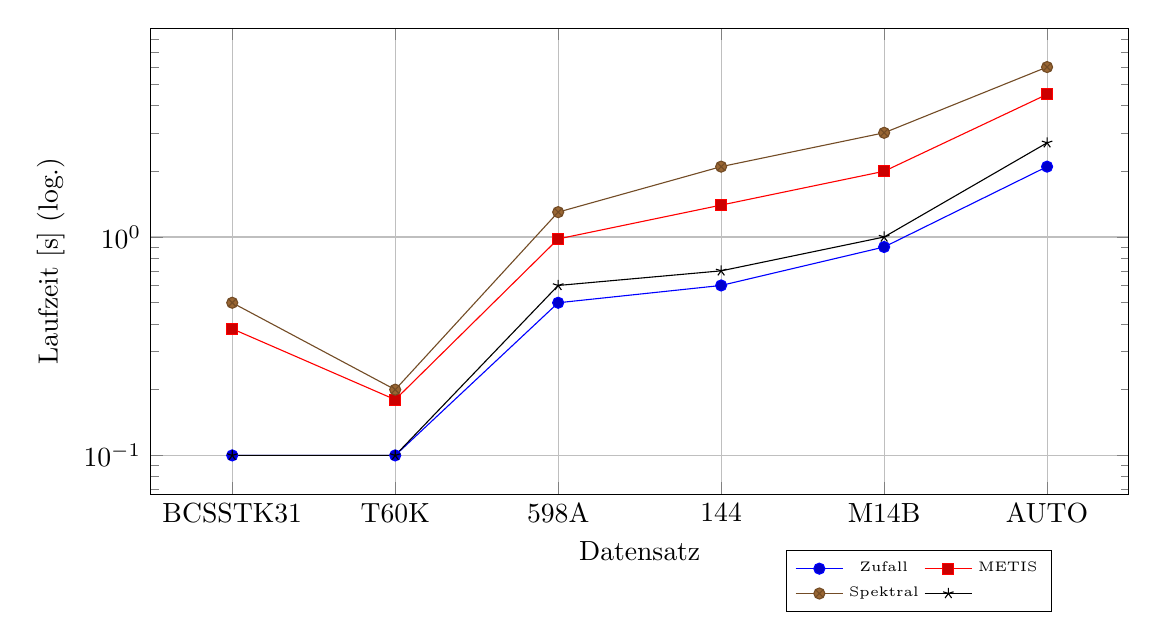
\begin{tikzpicture}
		\begin{axis}
		[grid=major,height=7.5cm,width=14cm,
		 legend style={legend pos=north west,font=\tiny,legend columns=2,at={(0.65,-0.12)}},
		 xlabel=Datensatz,ylabel={Laufzeit [s] (log.)},
		 x label style={align=center},
		 y label style={align=center},
		 %ybar,
		 ymode=log,
		 symbolic x coords={BCSSTK31,T60K,598A,144,M14B,AUTO},xtick=data]
			\addplot
				coordinates {
				(BCSSTK31,0.1)
				(T60K,0.1)
				(598A,0.5)
				(144,0.6)
				(M14B,0.9)
				(AUTO,2.1)
			};
			\addlegendentry{Zufall}
			\addplot
				coordinates {
				(BCSSTK31,0.38)
				(T60K,0.18)
				(598A,0.98)
				(144,1.4)
				(M14B,2)
				(AUTO,4.5)
			};
			\addlegendentry{METIS}
			\addplot
				coordinates {
				(BCSSTK31,0.5)
				(T60K,0.2)
				(598A,1.3)
				(144,2.1)
				(M14B,3)
				(AUTO,6)
			};
			\addlegendentry{Spektral}
			\addplot
				coordinates {
				(BCSSTK31,0.1)
				(T60K,0.1)
				(598A,0.6)
				(144,0.7)
				(M14B,1)
				(AUTO,2.7)
			};
			\addlegendentry{\kkmpp}
		\end{axis}
	\end{tikzpicture}
\caption{Laufzeiten der Algorithmen für Ratio Association mit $k = 128$.}
\label{fig:experiment-experiment-kkmpp-ratioassoc-runtime-128}
\end{figure}

\begin{figure}[h!]
	\centering
	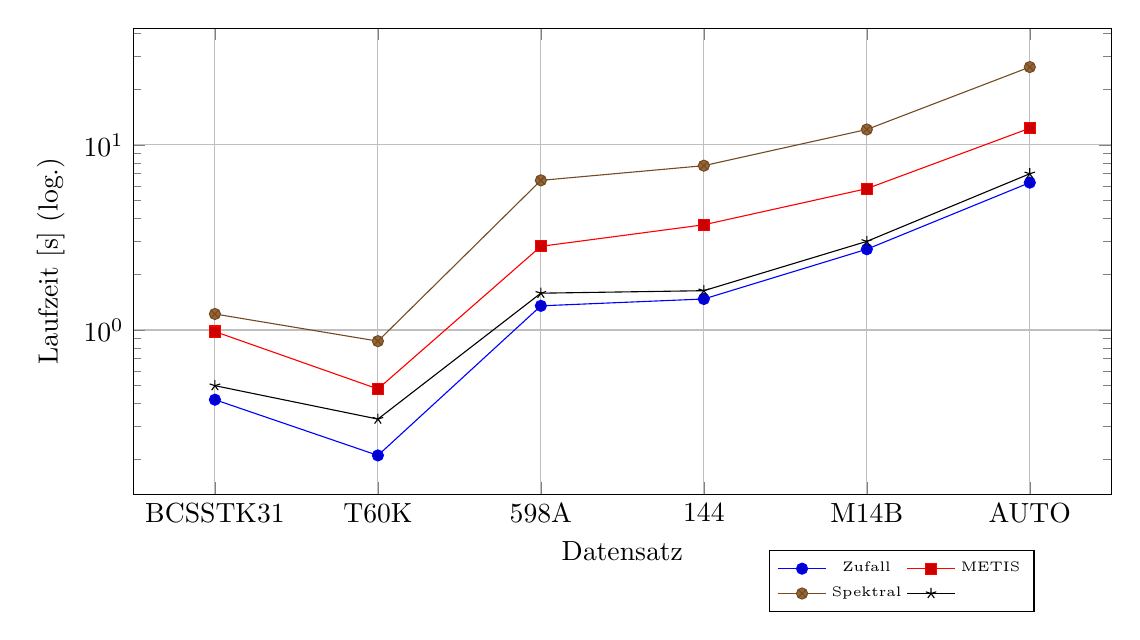
\begin{tikzpicture}
		\begin{axis}
		[grid=major,height=7.5cm,width=14cm,
		 legend style={legend pos=north west,font=\tiny,legend columns=2,at={(0.65,-0.12)}},
		 xlabel=Datensatz,ylabel={Laufzeit [s] (log.)},
		 x label style={align=center},
		 y label style={align=center},
		 %ybar,
		 ymode=log,
		 symbolic x coords={BCSSTK31,T60K,598A,144,M14B,AUTO},xtick=data]
			\addplot
				coordinates {
				(BCSSTK31,0.42)
				(T60K,0.21)
				(598A,1.35)
				(144,1.47)
				(M14B,2.73)
				(AUTO,6.25)
			};
			\addlegendentry{Zufall}
			\addplot
				coordinates {
				(BCSSTK31,0.98)
				(T60K,0.48)
				(598A,2.83)
				(144,3.7)
				(M14B,5.8)
				(AUTO,12.3)
			};
			\addlegendentry{METIS}
			\addplot
				coordinates {
				(BCSSTK31,1.22)
				(T60K,0.87)
				(598A,6.43)
				(144,7.72)
				(M14B,12.11)
				(AUTO,26.32)
			};
			\addlegendentry{Spektral}
			\addplot
				coordinates {
				(BCSSTK31,0.5)
				(T60K,0.33)
				(598A,1.58)
				(144,1.63)
				(M14B,3.01)
				(AUTO,6.98)
			};
			\addlegendentry{\kkmpp}
		\end{axis}
	\end{tikzpicture}
\caption{Laufzeiten der Algorithmen für Ratio Association mit $k = 512$.}
\label{fig:experiment-experiment-kkmpp-ratioassoc-runtime-512}
\end{figure}
\newpage
\begin{table}[t!]
\centering
\begin{tabular}{@{}ccccccc@{}} \toprule
	\textbf{Datensatz} & \textbf{Zufall} & \textbf{METIS} & \textbf{Spektral} & \textbf{Avg} & \textbf{Min} & \textbf{Max} \\ \midrule
	BCSSTK31 	& 0.1 & 0.38 & 0.51 & 0.1 & 0.1 & 0.1 \\
	T60K 		& 0.1 & 0.18 & 0.25 & 0.1 & 0.1 & 0.1 \\
	598A 		& 0.51 & 0.98 & 1.35 & 0.63 & 0.5 & 0.66 \\
	144 		& 0.62 & 1.43 & 2.16 & 0.74 & 0.6 & 0.91 \\
	M14B 		& 0.95 & 2.0 & 3 & 1.0 & 1.0 & 1.19 \\
	AUTO 		& 2.13 & 4.5 & 6 & 2.72 & 2.43 & 3.27 \\
	\bottomrule
\end{tabular}
\caption{Laufzeiten der Algorithmen für Ratio Association mit $k = 128$.}
\label{tbl:experiment-experiment-kkmpp-ratioassoc-runtime-128}
\end{table}

\begin{table}[h!]
\centering
\begin{tabular}{@{}ccccccc@{}} \toprule
	\textbf{Datensatz} & \textbf{Zufall} & \textbf{METIS} & \textbf{Spektral} & \textbf{Avg} & \textbf{Min} & \textbf{Max} \\ \midrule
	BCSSTK31 	& 0.42 & 0.98 & 1.22 & 0.5 & 0.47 & 0.71 \\
	T60K 		& 0.21 & 0.48 & 0.87 & 0.33 & 0.29 & 0.39 \\
	598A 		& 1.35 & 2.83 & 6.43 & 1.58 & 1.42 & 1.66 \\
	144 		& 1.47 & 3.7 & 7.72 & 1.63 & 1.55 & 1.74 \\
	M14B 		& 2.73 & 5.8 & 12.11 & 3.01 & 2.91 & 3.34 \\
	AUTO 		& 6.25 & 12.3 & 26.32 & 6.98 & 6.55 & 7.88 \\
	\bottomrule
\end{tabular}
\caption{Laufzeiten der Algorithmen für Ratio Association mit $k = 512$.}
\label{tbl:experiment-experiment-kkmpp-ratioassoc-runtime-512}
\end{table}

Sowohl für $k = 128$ als auch für $k = 512$ erfolgt die Ausführung mit zufälliger Initialisierung um mehr als einen Faktor von $2$
schneller als mit METIS oder spektralen Methoden. Die verbesserte Clusteringqualität erhalten wir bei beiden Verfahren unter
Einsatz von Rechenzeit, die nicht zu unterschätzen ist. Grundsätzlich ist zwar anzumerken, dass die erzielten Laufzeiten
generell sehr gering sind, wenn man bedenkt, dass die größten verwendeten Instanzen mehrere hunderttausend Knoten und einige
Millionen Kanten haben. Für die massenhafte Verarbeitung von Graphen dieser Größenordnung sind die Laufzeiteinbußen dennoch
beachtlich. Beim Algorithmus \kkmpp{} ist dagegen gut zu beobachten, dass die Laufzeiten kompetitiv zur rein zufälligen
Initialisierung sind. Der zusätzliche Overhead für die Kernel Methode entspricht relativ in etwa dem, was wir in den Experimenten
in Abschnitt~\ref{subsection:experiment-kernel-method} beobachten konnten. Insgesamt haben wir eine deutliche Verbesserung
erreicht, wenn man bedenkt, dass auch die Qualität der von \kkmpp{} berechneten Clusterings kompetitiv ist.

Zudem kann Abbildung~\ref{fig:experiment-experiment-kkmpp-ratioassoc-runtime-512} und
Tabelle~\ref{tbl:experiment-experiment-kkmpp-ratioassoc-runtime-512} entnommen werden, dass der Abstand zwischen dem spektralen
Verfahren und den anderen Methoden gerade bei großer Clusteranzahl $k$ mehrere Größenordnungen annimmt. Dies bestätigt
unsere zuvor formulierte Annahme, dass der Aufwand für die Berechnung der Eigenwerte für große Clusterzahlen sehr hoch wird.
Wir wollen am Ende dieses Abschnitts kurz die Verwendung von \kkmpp{} für die Bildsegmentierung thematisieren. Für die
Bildsegmentierung hat sich der Normalized Cut als geeignete Zielfunktion in der Graphpartitionierung erwiesen~\cite{ShiM00}.
Wir haben daher die Experimente auch für den Normalized Cut durchgeführt und stellen die Ergebnisse im Folgenden vor, bevor
wir uns der direkten Anwendung in der Bildsegmentierung widmen.

\begin{figure}[ht!]
	\centering
	\begin{tikzpicture}
		\begin{axis}
		[grid=major,height=7.5cm,width=14cm,
		 legend style={legend pos=north west,font=\tiny,legend columns=2,at={(0.65,-0.12)}},
		 xlabel=Datensatz,ylabel={Normalized Cut (log.)},
		 x label style={align=center},
		 y label style={align=center},
		 ybar,
		 ymode=log,
		 symbolic x coords={BCSSTK31,T60K,598A,144,M14B,AUTO},xtick=data]
			\addplot[fill=blue!40!white,postaction={pattern=north east lines}]
				coordinates {
				(BCSSTK31,29.2)
				(T60K,6.9)
				(598A,16.1)
				(144,15.3)
				(M14B,24.2)
				(AUTO,12.1)
			};
			\addlegendentry{Zufall}
			\addplot[fill=red!40!white,postaction={pattern=north west lines}]
				coordinates {
				(BCSSTK31,21.5)
				(T60K,5.4)
				(598A,14.3)
				(144,12.9)
				(M14B,21)
				(AUTO,9.9)
			};
			\addlegendentry{METIS}
			\addplot[fill=green!40!white,postaction={pattern=crosshatch}]
				coordinates {
				(BCSSTK31,19.8)
				(T60K,4.8)
				(598A,12.4)
				(144,10.3)
				(M14B,18.7)
				(AUTO,8.2)
			};
			\addlegendentry{Spektral}
			\addplot[fill=gray!40!white,postaction={pattern=crosshatch dots}]
				coordinates {
				(BCSSTK31,22)
				(T60K,5.8)
				(598A,13.5)
				(144,12.7)
				(M14B,21.7)
				(AUTO,9.5)
			};
			\addlegendentry{\kkmpp}
		\end{axis}
	\end{tikzpicture}
\caption{Normalized Cut Werte der Algorithmen für $k = 128$ (je kleiner, desto besser).}
\label{fig:experiment-experiment-kkmpp-ncut-128}
\end{figure}

\begin{figure}[ht!]
	\centering
	\begin{tikzpicture}
		\begin{axis}
		[grid=major,height=7.5cm,width=14cm,
		 legend style={legend pos=north west,font=\tiny,legend columns=2,at={(0.65,-0.12)}},
		 xlabel=Datensatz,ylabel={Normalized Cut (log.)},
		 x label style={align=center},
		 y label style={align=center},
		 ybar,
		 ymode=log,
		 symbolic x coords={BCSSTK31,T60K,598A,144,M14B,AUTO},xtick=data]
			\addplot[fill=blue!40!white,postaction={pattern=north east lines}]
				coordinates {
				(BCSSTK31,200.3)
				(T60K,58.2)
				(598A,124.7)
				(144,122.5)
				(M14B,112.6)
				(AUTO,98.3)
			};
			\addlegendentry{Zufall}
			\addplot[fill=red!40!white,postaction={pattern=north west lines}]
				coordinates {
				(BCSSTK31,160.4)
				(T60K,46.9)
				(598A,99.3)
				(144,94)
				(M14B,81)
				(AUTO,69.8)
			};
			\addlegendentry{METIS}
			\addplot[fill=green!40!white,postaction={pattern=crosshatch}]
				coordinates {
				(BCSSTK31,132.4)
				(T60K,37.3)
				(598A,87.5)
				(144,81.3)
				(M14B,72.7)
				(AUTO,62.5)
			};
			\addlegendentry{Spektral}
			\addplot[fill=gray!40!white,postaction={pattern=crosshatch dots}]
				coordinates {
				(BCSSTK31,172.3)
				(T60K,48.7)
				(598A,95.2)
				(144,93.3)
				(M14B,80.1)
				(AUTO,70)
			};
			\addlegendentry{\kkmpp}
		\end{axis}
	\end{tikzpicture}
\caption{Normalized Cut Werte der Algorithmen für $k = 512$ (je kleiner, desto besser).}
\label{fig:experiment-experiment-kkmpp-ncut-512}
\end{figure}
\newpage
\begin{table}
\centering
\begin{tabular}{@{}ccccccc@{}} \toprule
	\textbf{Datensatz} & \textbf{Zufall} & \textbf{METIS} & \textbf{Spektral} & \textbf{Avg} & \textbf{Min} & \textbf{Max} \\ \midrule
	BCSSTK31 	& 29.2 & 21.5 & 19.8 & 22 & 19.3 & 23.2 \\
	T60K 		& 6.9 & 5.4 & 4.8 & 5.8 & 5.1 & 6.3 \\
	598A 		& 16.1 & 14.3 & 12.4 & 13.5 & 13.1 & 13.9 \\
	144 		& 15.3 & 12.9 & 10.3 & 12.7 & 12.4 & 13.0 \\
	M14B 		& 24.2 & 21 & 18.7 & 21.7 & 21.1 & 22.6 \\
	AUTO 		& 12.1 & 9.9 & 8.2 & 9.5 & 8.9 & 10.1 \\
	\bottomrule
\end{tabular}
\caption{Normalized Cut Werte der Algorithmen für $k = 128$ (je kleiner, desto besser).}
\label{tbl:experiment-experiment-kkmpp-ncut-128}
\end{table}

\begin{table}[h!]
\centering
\begin{tabular}{@{}ccccccc@{}} \toprule
	\textbf{Datensatz} & \textbf{Zufall} & \textbf{METIS} & \textbf{Spektral} & \textbf{Avg} & \textbf{Min} & \textbf{Max} \\ \midrule
	BCSSTK31 	& 200.3 & 160.4 & 132.4 & 172.3 & 161.1 & 180.6 \\
	T60K 		& 58.2 & 46.9 & 37.3 & 48.7 & 45.2 & 51.3 \\
	598A 		& 124.7 & 99.3 & 87.5 & 95.2 & 90.3 & 100.9 \\
	144 		& 122.5 & 94 & 81.3 & 93.3 & 89.2 & 98.8 \\
	M14B 		& 112.6 & 81 & 72.7 & 80.1 & 71.2 & 87.8 \\
	AUTO 		& 98.3 & 69.8 & 62.5 & 70 & 64.3 & 76.2 \\
	\bottomrule
\end{tabular}
\caption{Normalized Cut Werte der Algorithmen für $k = 512$ (je kleiner, desto besser).}
\label{tbl:experiment-experiment-kkmpp-ncut-512}
\end{table}

\newpage

\begin{figure}[ht!]
	\centering
	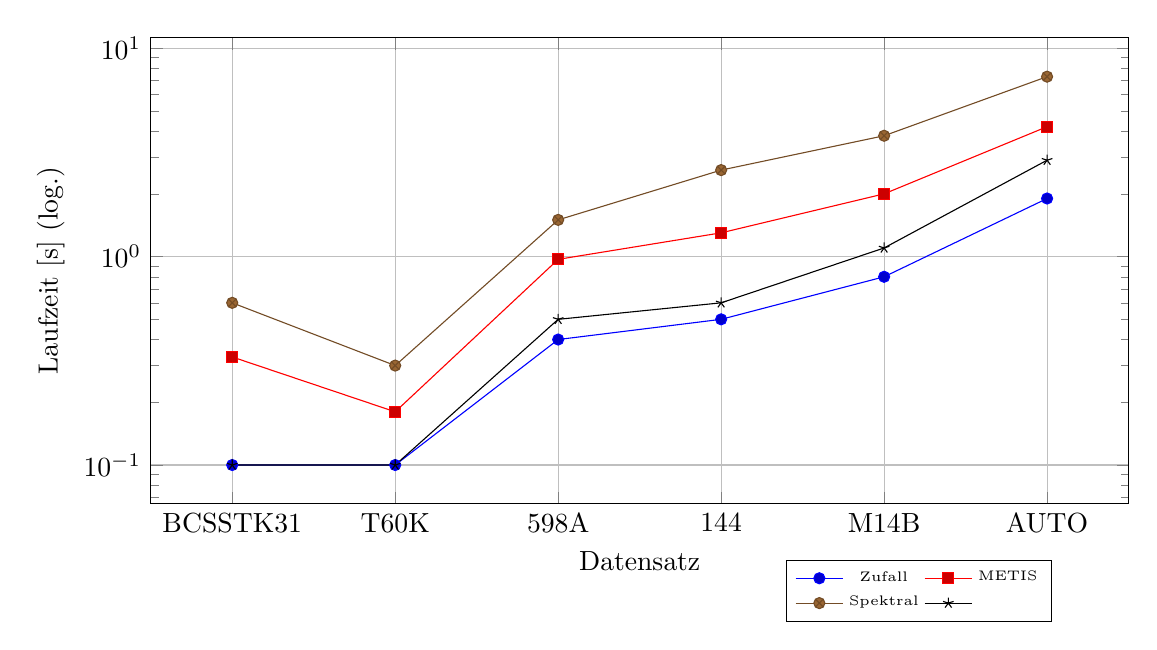
\begin{tikzpicture}
		\begin{axis}
		[grid=major,height=7.5cm,width=14cm,
		 legend style={legend pos=north west,font=\tiny,legend columns=2,at={(0.65,-0.12)}},
		 xlabel=Datensatz,ylabel={Laufzeit [s] (log.)},
		 x label style={align=center},
		 y label style={align=center},
		 %ybar,
		 ymode=log,
		 symbolic x coords={BCSSTK31,T60K,598A,144,M14B,AUTO},xtick=data]
			\addplot
				coordinates {
				(BCSSTK31,0.1)
				(T60K,0.1)
				(598A,0.4)
				(144,0.5)
				(M14B,0.8)
				(AUTO,1.9)
			};
			\addlegendentry{Zufall}
			\addplot
				coordinates {
				(BCSSTK31,0.33)
				(T60K,0.18)
				(598A,0.97)
				(144,1.3)
				(M14B,2)
				(AUTO,4.2)
			};
			\addlegendentry{METIS}
			\addplot
				coordinates {
				(BCSSTK31,0.6)
				(T60K,0.3)
				(598A,1.5)
				(144,2.6)
				(M14B,3.8)
				(AUTO,7.3)
			};
			\addlegendentry{Spektral}
			\addplot
				coordinates {
				(BCSSTK31,0.1)
				(T60K,0.1)
				(598A,0.5)
				(144,0.6)
				(M14B,1.1)
				(AUTO,2.9)
			};
			\addlegendentry{\kkmpp}
		\end{axis}
	\end{tikzpicture}
\caption{Laufzeiten der Algorithmen für Normalized Cut mit $k = 128$.}
\label{fig:experiment-experiment-kkmpp-ncut-runtime-128}
\end{figure}

\begin{figure}[h!]
	\centering
	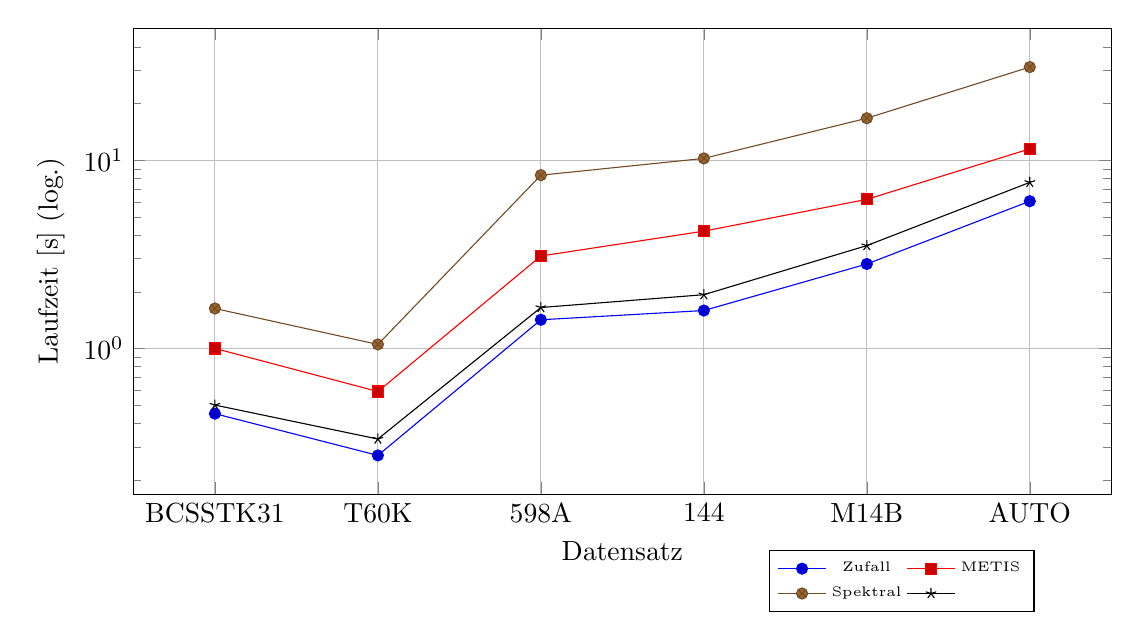
\begin{tikzpicture}
		\begin{axis}
		[grid=major,height=7.5cm,width=14cm,
		 legend style={legend pos=north west,font=\tiny,legend columns=2,at={(0.65,-0.12)}},
		 xlabel=Datensatz,ylabel={Laufzeit [s] (log.)},
		 x label style={align=center},
		 y label style={align=center},
		 %ybar,
		 ymode=log,
		 symbolic x coords={BCSSTK31,T60K,598A,144,M14B,AUTO},xtick=data]
			\addplot
				coordinates {
				(BCSSTK31,0.45)
				(T60K,0.27)
				(598A,1.42)
				(144,1.59)
				(M14B,2.81)
				(AUTO,6.06)
			};
			\addlegendentry{Zufall}
			\addplot
				coordinates {
				(BCSSTK31,1)
				(T60K,0.59)
				(598A,3.1)
				(144,4.2)
				(M14B,6.2)
				(AUTO,11.5)
			};
			\addlegendentry{METIS}
			\addplot
				coordinates {
				(BCSSTK31,1.63)
				(T60K,1.05)
				(598A,8.33)
				(144,10.23)
				(M14B,16.73)
				(AUTO,31.29)
			};
			\addlegendentry{Spektral}
			\addplot
				coordinates {
				(BCSSTK31,0.5)
				(T60K,0.33)
				(598A,1.65)
				(144,1.93)
				(M14B,3.52)
				(AUTO,7.63)
			};
			\addlegendentry{\kkmpp}
		\end{axis}
	\end{tikzpicture}
\caption{Laufzeiten der Algorithmen für Normalized Cut mit $k = 512$.}
\label{fig:experiment-experiment-kkmpp-ncut-runtime-512}
\end{figure}
\newpage
\begin{table}[t!]
\centering
\begin{tabular}{@{}ccccccc@{}} \toprule
	\textbf{Datensatz} & \textbf{Zufall} & \textbf{METIS} & \textbf{Spektral} & \textbf{Avg} & \textbf{Min} & \textbf{Max} \\ \midrule
	BCSSTK31 	& 0.1 & 0.33 & 0.6 & 0.1 & 0.1 & 0.1 \\
	T60K 		& 0.1 & 0.18 & 0.3 & 0.1 & 0.1 & 0.1 \\
	598A 		& 0.4 & 0.97 & 1.5 & 0.5 & 0.42 & 0.68 \\
	144 		& 0.5 & 1.3 & 2.6 & 0.6 & 0.53 & 0.93 \\
	M14B 		& 0.8 & 2.0 & 3.8 & 1.1 & 0.95 & 1.24 \\
	AUTO 		& 1.9 & 4.2 & 7.3 & 2.9 & 2.37 & 3.39 \\
	\bottomrule
\end{tabular}
\caption{Laufzeiten der Algorithmen für Normalized Cut mit $k = 128$.}
\label{tbl:experiment-experiment-kkmpp-ncut-runtime-128}
\end{table}

\begin{table}[h!]
\centering
\begin{tabular}{@{}ccccccc@{}} \toprule
	\textbf{Datensatz} & \textbf{Zufall} & \textbf{METIS} & \textbf{Spektral} & \textbf{Avg} & \textbf{Min} & \textbf{Max} \\ \midrule
	BCSSTK31 	& 0.45 & 1.0 & 1.63 & 0.5 & 0.48 & 0.77 \\
	T60K 		& 0.27 & 0.59 & 1.05 & 0.33 & 0.28 & 0.48 \\
	598A 		& 1.42 & 3.1 & 8.33 & 1.65 & 1.49 & 1.88 \\
	144 		& 1.59 & 4.2 & 10.23 & 1.93 & 1.66 & 1.98 \\
	M14B 		& 2.81 & 6.2 & 16.73 & 3.52 & 3.01 & 3.99 \\
	AUTO 		& 6.06 & 11.5 & 31.29 & 7.63 & 7.12 & 8.48 \\
	\bottomrule
\end{tabular}
\caption{Laufzeiten der Algorithmen für Normalized Cut mit $k = 512$.}
\label{tbl:experiment-experiment-kkmpp-ncut-runtime-512}
\end{table}

Die gemessenen Werte für den Normalized Cut sind in etwa in derselben relativen Größenordnung wie schon bei der 
Ratio Association. Qualitativ schneidet der Algorithmus \kkmpp{} nicht ganz so gut ab wie bei der Ratio Association, da
er hier auf keiner Instanz die spektrale Initialisierung verbessert. Bei der Laufzeit zeigen sich dafür aber besonders
deutliche Unterschiede. Insbesondere die spektrale Initialisierung ist bei den Experimenten mit großer Clusteranzahl
sehr deutlich abgeschlagen.
\paragraph{Bildsegmentierung.} Wir wollen abschließend wie angekündigt den \kkmpp-Algorithmus zur Bildsegmentierung einsetzen.
Dazu verwenden wir die Normalized Cut Zielfunktion und nutzen die MATLAB-Schnittstelle von Graclus, um die Cluster
graphisch zu plotten. Wir haben zu diesem Zweck die Grafiken zunächst mit Code für "`Image Segmentation with Normalized Cuts"' von
Jianbo Shi\footnote{\url{http://www.cis.upenn.edu/~jshi/software/} (Stand: 29.01.2015)} vorverarbeitet, wie in der
Graclus-Dokumentation beschrieben. Für die Gesichtserkennung bietet sich eine Clusteranzahl von $k = 2$ an. Die beiden
Cluster würden dann dem Gesicht und dem "`Rest"' des Bildes entsprechen. Die Experimente haben schnell gezeigt, dass sich für
die meisten Portrait-Fotos bessere Ergebnisse erzielen lassen, wenn $k = 3$ gewählt wird. In diesem Szenario entspricht wieder
ein Cluster dem Gesicht, ein weiteres Cluster den irrelevanten Teilen des Bildes, und ein drittes Cluster wird für
den Hals beziehungsweise den Torso verwendet.

\begin{figure}[t]
        \centering
        \begin{subfigure}[b]{0.5\textwidth}
        		\centering
                
\includegraphics[width=0.5\textwidth]{baby_0}
                \caption{Das vorverarbeitete, ursprüngliche Bild.}
                \label{fig:imageseg-kkmpp-k-3-a}
        \end{subfigure}%
        \begin{subfigure}[b]{0.5\textwidth}
        		\centering
                
\includegraphics[width=0.5\textwidth]{baby_1}
                \caption{Das erste Cluster (das Gesicht).}
                \label{fig:imageseg-kkmpp-k-3-b}
        \end{subfigure}
        \begin{subfigure}[b]{0.5\textwidth}
        		\centering
                
\includegraphics[width=0.5\textwidth]{baby_2}
                \caption{Das zweite Cluster (der Torso).}
                \label{fig:imageseg-kkmpp-k-3-c}
        \end{subfigure}%
        \begin{subfigure}[b]{0.5\textwidth}
        		\centering
                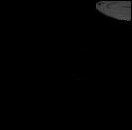
\includegraphics[width=0.5\textwidth]{baby_3}
                \caption{Das dritte Cluster (Fehler/Umgebung).}
                \label{fig:imageseg-kkmpp-k-3-d}
        \end{subfigure}
\caption{Mit \kkmpp{} segmentiertes Bild.}
\label{fig:imageseg-kkmpp}
\end{figure}
Abbildung~\ref{fig:imageseg-kkmpp} zeigt den graphischen Plot des berechneten Normalized Cut Clusterings von
Algorithmus \kkmpp. Auf den drei Clustern ist gut zu erkennen, dass unsere Clusteraufteilung hier gut funktioniert hat. Es
handelt sich um eine Beispielgrafik von der
Graclus-Webseite\footnote{\url{http://www.cs.utexas.edu/users/dml/Software/graclus.html} (Stand: 29.01.2015)}.
\absatz
Die Segmentierung einer einzelnen Grafik erfolgte nahezu unmittelbar. Um eine Vorstellung über die Leistungsfähigkeit des
Algorithmus in der Bildsegmentierung zu ermöglichen, haben wir ihn auf die
Extended Yale Face Database B (B+)\footnote{\url{http://vision.ucsd.edu/content/extended-yale-face-database-b-b}\\
(Stand: 29.01.2015)}~\cite{GeorghiadesBK01} angewandt. Dabei handelt es sich um eine Sammlung von 16128 Portrait-Fotos von
28 Menschen in 9 unterschiedlichen Positionen und 64 verschiedenen Belichtungsszenarien. Der gesamte Datensatz ist etwa
2 GB groß. Der Datensatz konnte mit \kkmpp{} in rund 50 Minuten verarbeitet werden. Unter Einsatz von METIS und mit
der spektralen Initialisierung dauerte die gesamte Verarbeitung rund 2 Stunden und 10 Minuten, also mehr als doppelt so lange.
Die "`Korrektheit"' der Gesichtserkennung konnte wegen der Anzahl der Bilder nicht vollständig ermittelt werden, da diese nur
durch menschlichen Augenschein verifiziert werden kann. Es ist nötig, bei einer Segmentierung zu prüfen, ob ein Cluster
dem Gesicht auf dem Foto entspricht.
In einer Stichprobe von 160 Bildern wurden 153 Bilder korrekt segmentiert, das entspricht einem Anteil von 96\%.
Bei der spektralen Methode wurden 157 Bilder korrekt segmentiert, was einem Anteil von 98\% entspricht.

\subsection{Die Kernmengenkonstruktion}
\label{subsection:experiment-coreset}

Unsere Variante der Kernmengenkonstruktion nennen wir in diesem Abschnitt verkürzt \CsTwo.

\subsubsection{\texorpdfstring{$k$}{k}-means mit der Kernmengenkonstruktion}
Die empirische Evaluation der "`Güte"' einer~(starken)~Kernmenge im Sinne ihrer Definition~\ref{def:strong-coreset}
beziehungsweise~\ref{def:coreset-with-offset} ist im Allgemeinen schwierig, da sich schlecht für alle möglichen Zentrenmengen
die jeweiligen Kosten vergleichen lassen. Neben der Messung der Laufzeiten geht man bezüglich der Qualitätsanalyse von Kernmengen
wie beispielsweise in~\cite{AckermannMRSLS12,FichtenbergerGSSS13} vor. Man berechnet einerseits die Kernmenge $S$ für die
Eingabepunktmenge $P$, wendet auf $S$ einen $k$-means-Algorithmus an und erhält eine Menge von $k$ Zentren
$C^1 = \{c_1^1, \dots, c_k^1\}$, für die sich $k$-means-Kosten $c^1$ in Bezug auf die Eingabepunktmenge $P$ ergeben.
Andererseits wendet man denselben $k$-means-Algorithmus direkt auf ganz $P$ an und erhält ebenfalls eine Zentrenmenge
$C^2 = \{c_1^2, \dots, c_k^2\}$, für die sich $k$-means-Kosten $c^2$ für $P$ ergeben. Die $k$-means-Kosten $c^1$ und $c^2$ lassen
sich vergleichen. Die untersuchte Qualität der Kernmenge bezieht sich bei diesem Vorgehen dann auf die Lösung des
$k$-means-Problems mit Hilfe der Kernmenge.
\absatz
Auf diese Weise wollen wir in diesem Abschnitt vorgehen. Dazu haben wir auf die Ausgaben der Kernmengen-Algorithmen,
die wir jeweils zehnmal ausgeführt haben, den $k$-means-Algorithmus und den \kmpp-Algorithmus je zehnmal angewandt und die
durchschnittlichen Kosten für den Vergleich genommen. Insgesamt wurden also 100 Ausführungen inklusive anschließendem $k$-means und
weitere 100 Ausführungen mit anschließendem \kmpp{} gemessen.
Diese Methode der Evaluation ist zwar nicht allumfassend, wir können jedoch den gesamten Algorithmus evaluieren und insbesondere
die Leistungsfähigkeit der Kernmengenkonstruktion zur Lösung des $k$-means-Problems bewerten.
\paragraph{Algorithmen.} Für einen Vergleich ziehen wir zunächst die Kernmengenkonstruktionen BICO~\cite{FichtenbergerGSSS13}
und \Skmpp~\cite{AckermannMRSLS12} heran. Beide Algorithmen sind state-of-the-art Datenstromalgorithmen zur Berechnung von
Kernmengen. Außerdem wollen wir auch hier wieder die Dlib-Implementierung von \kmpp{} zum Vergleich einsetzen, da wir in
unserer Konstruktion intensiven Gebrauch von der $D^2$-Gewichtung machen.
\paragraph{Datensätze.} Sowohl \kmpp{} als auch \CsTwo{} benötigen im Vergleich zu den Datenstromalgorithmen bereits auf Instanzen
mit mehreren hunderttausend Punkten vergleichsweise lange Ausführungszeiten. Wir beschränken uns daher in diesem Teil der
Evaluation auf mittelgroße Instanzen mit weniger als $10^6$ Punkten und insbesondere überschaubarer Dimensionsanzahl (bis
ca. $50$ Dimensionen). Tabelle~\ref{tbl:experiment-coresets-datasets} zeigt die Eigenschaften der ausgewählten Datensätze aus dem
UCI Machine Learning Repository.

\begin{table}[t]
\centering
\begin{tabular}{@{}ccc@{}} \toprule
	\textbf{Datensatz} & \textbf{Anzahl Punkte} & \textbf{Dimension} $d$ \\ \midrule
	Spambase & 4601 & 57 \\
	NYSK & 10421  & 7 \\
	Intrusion / KDD Cup 1999~\cite{AckermannMRSLS12} & 311078 & 34 \\
	Covertype & 581012 & 54 \\ \bottomrule
\end{tabular}
\caption{Eigenschaften der Datensätze aus~\cite{Lichman13} für die Evaluation von~\CsTwo.}
\label{tbl:experiment-coresets-datasets}
\end{table}

\paragraph{Kernmengen-Größe.}
Eine asymptotische Größe von $\mathcal{O}(k)$ ist eine natürliche untere Schranke für die Größe einer Kernmenge, die wir
erreichen wollen. Wir orientieren uns in unseren Experimenten an~\cite{AckermannMRSLS12,FichtenbergerGSSS13}. In beiden Papieren
wurden in der experimentellen Auswertungen Kernmengen der Größe $200k$ konstruiert. Für die beiden Datensätze Spambase und
NYSK würden die Kernmengen bei einer Größe von $200k$ mehr Punkte enthalten als die Ursprungsmenge. Bei diesen beiden Datensätzen
haben wir daher Kernmengen der Größe $20k$ berechnet, um mehr Testwerte für einen umfassenderen Vergleich zu generieren, sofern
die Wahl der Parameter dies zulässt (insbesondere $c \leq 20$).
Für die Evaluation unserer Konstruktion ergibt sich die Herausforderung, die diversen Parameter so zu wählen, dass die
berechnete Kernmenge in etwa diese Größe annimmt. Wir können dies auf mehreren Wegen erreichen. Es ist beispielsweise möglich,
schon bei der initialen Partitionierung ein großes $c$ zu wählen (im Extremfall sogar schon hier $c=200$) und durch die maximale
Tiefe oder den Kostenfaktor $f$ dafür zu sorgen, dass nur bis zu einer geringen Tiefe partitioniert wird (oder im Extremfall
gar nicht weiter partitioniert wird). Alternativ können wir auch ein kleines $c$ wählen und dafür größere
Werte von $d$ wählen, sodass wir initial nur wenige Teilmengen haben und in der rekursiven Partitionierung eine größere
Anzahl von Teilmengen erzielen.
\paragraph{Clusteranzahl.} Wir wollen auch hier mit verschiedenen Werten für die Clusteranzahl $k$ arbeiten.
Dabei orientieren wir uns an den Experimenten aus~\cite{AckermannMRSLS12,FichtenbergerGSSS13}. Wir führen die Algorithmen
jeweils mit $k \in \{ 10, 30, 50 \}$ aus.
\absatz
Wir geben bei den Ergebnistabellen immer den durchschnittlichen Wert für Kosten und Laufzeit von zehn Ausführungen
des $k$-means-Algorithmus beziehungsweise des \kmpp-Algorithmus für je zehn Ausführungen der Kernmengen-Algorithmen an.
Bei den Kernmengen-Algorithmen beziehen sich diese Werte auf die Ausführung von $k$-means beziehungsweise \kmpp{} unter
Eingabe der Kernmenge und bei $k$-means beziehungsweise \kmpp{} selbst auf die 100 Ausführungen auf der gesamten Punktmenge $P$.
Für \CsTwo{} geben wir die jeweiligen Parameter im Namen des Algorithmus an. Beispielsweise schreiben wir für
$c = 200$, $d=/$, $f=/$ und $T=1$: \CsTwo-c-200-d-/-f-/-T-1.
Die Wahl von $d$ und $f$ ist hier irrelevant, da wegen $T$ nur initial partitioniert wird. Dies deuten wir mit der
Notation "`/"' an.

Wir betrachten zunächst die Ergebnisse der Kernmengenkonstruktionen mit anschließender Ausführung des $k$-means-Algorithmus im
Vergleich zu \kmpp.
\newpage
\begin{table}[h]
\centering
\begin{tabular}{@{}cccccc@{}} \toprule
	\textbf{Algorithmus} & $k$ & \multicolumn{4}{c}{\textbf{Datensatz}} \\
	\cmidrule(r){3-6} & 		& Spambase 				& NYSK 				& Intrusion 			& Covertype \\ \toprule
	\Skmpp 						& 10 & $8.44 \cdot 10^7$ & $5.93 \cdot 10^8$ & $1.58 \cdot 10^{13}$ & $3.77 \cdot 10^{11}$ \\
		 						& 30 & $1.33 \cdot 10^7$ & $4.76 \cdot 10^8$ & $4.63 \cdot 10^{11}$ & $1.72 \cdot 10^{11}$ \\
		 						& 50 & $6.57 \cdot 10^6$ & $6.63 \cdot 10^8$ & $1.22 \cdot 10^{11}$ & $1.29 \cdot 10^{11}$ \\
	\midrule
	BICO 						& 10 & $7.21 \cdot 10^7$ & $5.71 \cdot 10^8$ & $1.37 \cdot 10^{13}$ & $3.56 \cdot 10^{11}$ \\
			 					& 30 & $1.29 \cdot 10^7$ & $4.45 \cdot 10^8$ & $4.48 \cdot 10^{11}$ & $1.59 \cdot 10^{11}$ \\
		 						& 50 & $6.33 \cdot 10^6$ & $6.32 \cdot 10^8$ & $1.18 \cdot 10^{11}$ & $1.15 \cdot 10^{11}$ \\
	\midrule
	\kmpp 						& 10 & $8.71 \cdot 10^7$ & $6.09 \cdot 10^8$ & $1.75 \cdot 10^{13}$ & $3.42 \cdot 10^{11}$ \\
			 					& 30 & $1.34 \cdot 10^7$ & $4.98 \cdot 10^8$ & $4.96 \cdot 10^{11}$ & $1.54 \cdot 10^{11}$ \\
		 						& 50 & $6.68 \cdot 10^6$ & $7.01 \cdot 10^8$ & $1.29 \cdot 10^{11}$ & $1.13 \cdot 10^{11}$ \\
	\midrule
	\CsTwo-c-200-d-/-f-/-T-1	& 10 & $8.95 \cdot 10^7$ & $6.42 \cdot 10^8$ & $1.82 \cdot 10^{13}$ & $3.55 \cdot 10^{11}$ \\
			 					& 30 & - 				& $5.33 \cdot 10^8$ & $4.95 \cdot 10^{11}$ & $1.70 \cdot 10^{11}$ \\
		 						& 50 & - 				& $7.67 \cdot 10^8$	& $1.32 \cdot 10^{11}$ & $1.18 \cdot 10^{11}$ \\
	\midrule
	\CsTwo-c-1-d-50-f-1.3-T-3	& 10 & $8.61 \cdot 10^7$ & $6.17 \cdot 10^8$ & $1.82 \cdot 10^{13}$ & $3.52 \cdot 10^{11}$ \\
			 					& 30 & $1.42 \cdot 10^7$ & $5.06 \cdot 10^8$ & $4.89 \cdot 10^{11}$ & $1.63 \cdot 10^{11}$ \\
		 						& 50 & $6.71 \cdot 10^6$ & $7.02 \cdot 10^8$ & $1.31 \cdot 10^{11}$ & $1.14 \cdot 10^{11}$ \\
	\midrule
	\CsTwo-c-5-d-25-f-1.2-T-15	& 10 & $8.85 \cdot 10^7$ & $6.32 \cdot 10^8$ & $1.98 \cdot 10^{13}$ & $3.62 \cdot 10^{11}$ \\
			 					& 30 & $1.49 \cdot 10^7$ & $5.16 \cdot 10^8$ & $5.11 \cdot 10^{11}$ & $1.64 \cdot 10^{11}$ \\
		 						& 50 & $6.91 \cdot 10^6$ & $7.18 \cdot 10^8$ & $1.41 \cdot 10^{11}$ & $1.19 \cdot 10^{11}$ \\
	\midrule
	\CsTwo-c-50-d-10-f-1.4-T-10	& 10 & $8.60 \cdot 10^7$ & $5.99 \cdot 10^8$ & $1.70 \cdot 10^{13}$ & $3.51 \cdot 10^{11}$ \\
			 					& 30 & $1.36 \cdot 10^7$ & $5.02 \cdot 10^8$ & $4.93 \cdot 10^{11}$ & $1.61 \cdot 10^{11}$ \\
		 						& 50 & $6.74 \cdot 10^6$ & $7.04 \cdot 10^8$ & $1.32 \cdot 10^{11}$ & $1.17 \cdot 10^{11}$ \\
	\midrule
	\CsTwo-c-100-d-5-f-1.1-T-4	& 10 & $8.93 \cdot 10^7$ & $6.40 \cdot 10^8$ & $1.80 \cdot 10^{13}$ & $3.51 \cdot 10^{11}$ \\
			 					& 30 & $1.48 \cdot 10^7$ & $5.26 \cdot 10^8$ & $5.01 \cdot 10^{11}$ & $1.64 \cdot 10^{11}$ \\
		 						& 50 & - 				& $7.49 \cdot 10^8$ & $1.31 \cdot 10^{11}$ & $1.18 \cdot 10^{11}$ \\
	\bottomrule
\end{tabular}
\caption{Durchschnittliche Kosten der Algorithmen für $k \in \{ 10, 30, 50 \}$ (je kleiner, desto besser). Bei den
Kernmengen-Algorithmen wurde anschließend der $k$-means-Algorithmus ausgeführt.}
\label{tbl:experiment-coresets-costs-kmeans}
\end{table}
\newpage
\begin{table}[h]
\centering
\begin{tabular}{@{}cccccc@{}} \toprule
	\textbf{Algorithmus} & $k$ & \multicolumn{4}{c}{\textbf{Datensatz}} \\
	\cmidrule(r){3-6} & 		& Spambase 				& NYSK 				& Intrusion 			& Covertype \\ \toprule
	\Skmpp 						& 10 & $3.2$ 			& $4.1$ 			& $71.6$ 				& $241.8$ \\
		 						& 30 & $16.1$ 			& $20.2$ 			& $98.1$ 				& $381.7$ \\
		 						& 50 & $44.1$ 			& $67.3$ 			& $230.3$ 				& $529.0$ \\
	\midrule
	BICO 						& 10 & $0.1$ 			& $1.5$ 			& $15.2$ 				& $25.2$ \\
			 					& 30 & $0.1$ 			& $2.0$ 			& $17.1$ 				& $45.7$ \\
		 						& 50 & $0.1$ 			& $2.4$ 			& $20.5$ 				& $42.3$ \\
	\midrule
	\kmpp 						& 10 & $1.2$ 			& $2.9$ 			& $23.8$ 				& $181.2$ \\
			 					& 30 & $5.7$ 			& $10.2$ 			& $897.3$ 				& $2024.7$ \\
		 						& 50 & $13.3$ 			& $28.3$ 			& $644.0$ 				& $6922.9$ \\
	\midrule
	\CsTwo-c-200-d-/-f-/-T-1	& 10 & $3.1$			& $7.2$				& $48.4$ 				& $381.2$ \\
			 					& 30 & - 				& $21.1$			& $1574.1$ 				& $4003.3$ \\
		 						& 50 & - 				& $58.6$			& $1309.2$ 				& $12372.3$ \\
	\midrule
	\CsTwo-c-1-d-50-f-1.3-T-3	& 10 & $2.0$ 			& $5.8$ 			& $40.9$ 				& $321.9$ \\
			 					& 30 & $11.4$ 			& $19.7$ 			& $1703.3$ 				& $3321.6$ \\
		 						& 50 & $25.7$ 			& $55.4$ 			& $1122.1$ 				& $11242.1$ \\
	\midrule
	\CsTwo-c-5-d-25-f-1.2-T-15	& 10 & $1.9$ 			& $5.1$ 			& $40.3$ 				& $299.7$ \\
			 					& 30 & $10.7$ 			& $15.7$ 			& $1603.8$ 				& $2812.7$ \\
		 						& 50 & $24.3$ 			& $44.2$ 			& $1078.1$ 				& $9659.8$ \\
	\midrule
	\CsTwo-c-50-d-10-f-1.4-T-10	& 10 & $1.6$ 			& $3.0$ 			& $35.3$ 				& $239.0$ \\
			 					& 30 & $8.2$ 			& $13.5$ 			& $1237.9$ 				& $2044.4$ \\
		 						& 50 & $17.8$ 			& $38.2$ 			& $851.2$ 				& $7831.1$ \\
	\midrule
	\CsTwo-c-100-d-5-f-1.1-T-4	& 10 & $2.1$ 			& $17.2$ 			& $41.1$ 				& $331.0$ \\
			 					& 30 & $9.8$ 			& $16.9$			& $1787.7$ 				& $3912.7$ \\
		 						& 50 & - 				& $24.7$ 			& $1129.5$ 				& $10265.0$ \\
	\bottomrule
\end{tabular}
\caption{Durchschnittliche Laufzeiten der Algorithmen für $k \in \{ 10, 30, 50 \}$ in Sekunden. Bei den Kernmengen-Algorithmen
wurde anschließend der $k$-means-Algorithmus ausgeführt.}
\label{tbl:experiment-coresets-runtime-kmeans}
\end{table}
Der Kostenübersicht in Tabelle~\ref{tbl:experiment-coresets-costs-kmeans} können wir entnehmen, dass die Datenstromalgorithmen
mit Ausnahme von Covertype geringere Kosten erzielen als \kmpp. Auf Covertype sind die Kosten jedoch nur geringfügig größer.
Im Schnitt erzielt \Skmpp{} etwa 2-3\% geringere Kosten, während BICO bis zu 5\% geringere Kosten erzielt. \CsTwo{} hingegen
erreicht in drei Parametrisierungen rund 3\% höhere Kosten. Die besten Werte werden bei $c=1, d=50$ und $c=50, d=10$ erzielt.
Bei letzteren ist \CsTwo{} etwa 2\% besser als \kmpp{} aber noch leicht über den Werten von \Skmpp.
Bei den Laufzeiten in Tabelle~\ref{tbl:experiment-coresets-runtime-kmeans} ist die Ordnung der Algorithmen gleich.
Wir können jedoch insbesondere bei den Datenstromalgorithmen einen massiven Unterschied von einigen Größenordnungen in der
Laufzeit ausmachen. Die Datenstromalgorithmen sind deutlich schneller als \kmpp{} und die Kernmengenkonstruktion.
\CsTwo{} erzielt hier die geringsten Laufzeiten bei $c=50, d=10$, ist jedoch im Schnitt immer noch ca. 10-15\% langsamer als \kmpp.

Wir betrachten als nächstes die Ergebnisse Kernmengen-Algorithmen bei anschließender Ausführung von \kmpp.
\begin{table}[h]
\centering
\begin{tabular}{@{}cccccc@{}} \toprule
	\textbf{Algorithmus} & $k$ & \multicolumn{4}{c}{\textbf{Datensatz}} \\
	\cmidrule(r){3-6} & 		& Spambase 				& NYSK 				& Intrusion 			& Covertype \\ \toprule
	\Skmpp 						& 10 & $7.85 \cdot 10^7$ & $5.67 \cdot 10^8$ & $1.27 \cdot 10^{13}$ & $3.43 \cdot 10^{11}$ \\
		 						& 30 & $1.24 \cdot 10^7$ & $4.22 \cdot 10^8$ & $4.29 \cdot 10^{11}$ & $1.57 \cdot 10^{11}$ \\
		 						& 50 & $6.29 \cdot 10^6$ & $6.12 \cdot 10^8$ & $1.11 \cdot 10^{11}$ & $1.15 \cdot 10^{11}$ \\
	\midrule
	BICO 						& 10 & $7.81 \cdot 10^7$ & $5.52 \cdot 10^8$ & $1.19 \cdot 10^{13}$ & $3.22 \cdot 10^{11}$ \\
			 					& 30 & $1.22 \cdot 10^7$ & $4.13 \cdot 10^8$ & $4.25 \cdot 10^{11}$ & $1.48 \cdot 10^{11}$ \\
		 						& 50 & $6.15 \cdot 10^6$ & $5.98 \cdot 10^8$ & $1.03 \cdot 10^{11}$ & $1.02 \cdot 10^{11}$ \\
	\midrule
	\kmpp 						& 10 & $8.71 \cdot 10^7$ & $6.09 \cdot 10^8$ & $1.75 \cdot 10^{13}$ & $3.42 \cdot 10^{11}$ \\
			 					& 30 & $1.34 \cdot 10^7$ & $4.98 \cdot 10^8$ & $4.96 \cdot 10^{11}$ & $1.54 \cdot 10^{11}$ \\
		 						& 50 & $6.68 \cdot 10^6$ & $7.01 \cdot 10^8$ & $1.29 \cdot 10^{11}$ & $1.13 \cdot 10^{11}$ \\
	\midrule
	\CsTwo-c-200-d-/-f-/-T-1	& 10 & $8.71 \cdot 10^7$ & $6.07 \cdot 10^8$ & $1.63 \cdot 10^{13}$ & $3.35 \cdot 10^{11}$ \\
			 					& 30 & - 				& $4.96 \cdot 10^8$ & $4.82 \cdot 10^{11}$ & $1.51 \cdot 10^{11}$ \\
		 						& 50 & - 				& $7.00 \cdot 10^8$	& $1.23 \cdot 10^{11}$ & $1.09 \cdot 10^{11}$ \\
	\midrule
	\CsTwo-c-1-d-50-f-1.3-T-3	& 10 & $8.33 \cdot 10^7$ & $5.92 \cdot 10^8$ & $1.59 \cdot 10^{13}$ & $3.31 \cdot 10^{11}$ \\
			 					& 30 & $1.30 \cdot 10^7$ & $4.88 \cdot 10^8$ & $4.75 \cdot 10^{11}$ & $1.48 \cdot 10^{11}$ \\
		 						& 50 & $6.59 \cdot 10^6$ & $6.89 \cdot 10^8$ & $1.19 \cdot 10^{11}$ & $1.06 \cdot 10^{11}$ \\
	\midrule
	\CsTwo-c-5-d-25-f-1.2-T-15	& 10 & $8.63 \cdot 10^7$ & $6.00 \cdot 10^8$ & $1.71 \cdot 10^{13}$ & $3.40 \cdot 10^{11}$ \\
			 					& 30 & $1.33 \cdot 10^7$ & $4.94 \cdot 10^8$ & $4.89 \cdot 10^{11}$ & $1.51 \cdot 10^{11}$ \\
		 						& 50 & $6.65 \cdot 10^6$ & $6.97 \cdot 10^8$ & $1.25 \cdot 10^{11}$ & $1.10 \cdot 10^{11}$ \\
	\midrule
	\CsTwo-c-50-d-10-f-1.4-T-10	& 10 & $8.22 \cdot 10^7$ & $5.85 \cdot 10^8$ & $1.52 \cdot 10^{13}$ & $3.30 \cdot 10^{11}$ \\
			 					& 30 & $1.28 \cdot 10^7$ & $4.80 \cdot 10^8$ & $4.70 \cdot 10^{11}$ & $1.47 \cdot 10^{11}$ \\
		 						& 50 & $6.49 \cdot 10^6$ & $6.81 \cdot 10^8$ & $1.17 \cdot 10^{11}$ & $1.09 \cdot 10^{11}$ \\
	\midrule
	\CsTwo-c-100-d-5-f-1.1-T-4	& 10 & $8.70 \cdot 10^7$ & $6.04 \cdot 10^8$ & $1.73 \cdot 10^{13}$ & $3.42 \cdot 10^{11}$ \\
			 					& 30 & $1.32 \cdot 10^7$ & $4.95 \cdot 10^8$ & $4.92 \cdot 10^{11}$ & $1.54 \cdot 10^{11}$ \\
		 						& 50 & - 				& $6.97 \cdot 10^8$ & $1.28 \cdot 10^{11}$ & $1.12 \cdot 10^{11}$ \\
	\bottomrule
\end{tabular}
\caption{Durchschnittliche Kosten der Algorithmen für $k \in \{ 10, 30, 50 \}$ (je kleiner, desto besser). Bei den
Kernmengen-Algorithmen wurde anschließend der \kmpp-Algorithmus ausgeführt.}
\label{tbl:experiment-coresets-costs-kmpp}
\end{table}
\newpage
\begin{table}[h]
\centering
\begin{tabular}{@{}cccccc@{}} \toprule
	\textbf{Algorithmus} & $k$ & \multicolumn{4}{c}{\textbf{Datensatz}} \\
	\cmidrule(r){3-6} & 		& Spambase 				& NYSK 				& Intrusion 			& Covertype \\ \toprule
	\Skmpp 						& 10 & $1.4$ 			& $2.7$ 			& $28.7$ 				& $115.2$ \\
		 						& 30 & $6.3$ 			& $9.3$ 			& $45.3$ 				& $170.5$ \\
		 						& 50 & $18.2$ 			& $25.2$ 			& $100.1$ 				& $290.2$ \\
	\midrule
	BICO 						& 10 & $0.1$ 			& $0.8$ 			& $7.6$ 				& $13.7$ \\
			 					& 30 & $0.1$ 			& $0.9$ 			& $9.8$ 				& $16.3$ \\
		 						& 50 & $0.1$ 			& $1.0$ 			& $12.1$ 				& $19.2$ \\
	\midrule
	\kmpp 						& 10 & $1.2$ 			& $2.9$ 			& $23.8$ 				& $181.2$ \\
			 					& 30 & $5.7$ 			& $10.2$ 			& $897.3$ 				& $2024.7$ \\
		 						& 50 & $13.3$ 			& $28.3$ 			& $644.0$ 				& $6922.9$ \\
	\midrule
	\CsTwo-c-200-d-/-f-/-T-1	& 10 & $1.2$			& $2.9$				& $22.6$ 				& $175.3$ \\
			 					& 30 & - 				& $10.0$			& $854.2$ 				& $1889.1$ \\
		 						& 50 & - 				& $27.8$			& $608.1$ 				& $6122.3$ \\
	\midrule
	\CsTwo-c-1-d-50-f-1.3-T-3	& 10 & $1.1$ 			& $2.5$ 			& $21.1$ 				& $155.3$ \\
			 					& 30 & $5.5$ 			& $9.1$ 			& $802.3$ 				& $1772.4$ \\
		 						& 50 & $12.9$ 			& $26.5$ 			& $577.2$ 				& $5532.1$ \\
	\midrule
	\CsTwo-c-5-d-25-f-1.2-T-15	& 10 & $1.0$ 			& $2.3$ 			& $19.9$ 				& $149.2$ \\
			 					& 30 & $5.2$ 			& $8.3$ 			& $763.7$ 				& $1566.3$ \\
		 						& 50 & $11.8$ 			& $23.2$ 			& $522.3$ 				& $5138.4$ \\
	\midrule
	\CsTwo-c-50-d-10-f-1.4-T-10	& 10 & $0.9$ 			& $1.8$ 			& $18.1$ 				& $121.3$ \\
			 					& 30 & $4.3$ 			& $7.6$ 			& $653.2$ 				& $1132.5$ \\
		 						& 50 & $9.9$ 			& $20.4$ 			& $434.1$ 				& $4237.2$ \\
	\midrule
	\CsTwo-c-100-d-5-f-1.1-T-4	& 10 & $1.0$ 			& $8.5$ 			& $20.6$ 				& $162.4$ \\
			 					& 30 & $5.1$ 			& $8.0$				& $788.1$ 				& $1802.4$ \\
		 						& 50 & - 				& $24.7$ 			& $554.3$ 				& $5322.1$ \\
	\bottomrule
\end{tabular}
\caption{Durchschnittliche Laufzeiten der Algorithmen für $k \in \{ 10, 30, 50 \}$ in Sekunden. Bei den
Kernmengen-Algorithmen wurde anschließend der \kmpp-Algorithmus ausgeführt.}
\label{tbl:experiment-coresets-runtime-kmpp}
\end{table}
Mit der anschließenden Ausführung von \kmpp{} erzielen sämtliche Kernmengen-Algorithmen bezüglich $k$-means-Kosten und
Laufzeiten bessere Ergebnisse. Die Verbesserung reicht bei den Kosten von 5-10\% und bei den Laufzeiten bis zu einer Halbierung
der Laufzeiten.
Tabelle~\ref{tbl:experiment-coresets-costs-kmpp} ist zu entnehmen, dass unsere Konstruktion mit allen Parametrisierungen bessere
$k$-means-Kosten erzielt als \kmpp. In der Spitze sind Verbesserungen von bis zu 10\% zu verzeichnen. Andererseits erzielen
die Datenstromalgorithmen \Skmpp und BICO durchweg noch geringere Kosten (in der Spitze bis rund 20\% weniger im Vergleich
zu \kmpp). Bei den Laufzeiten in Tabelle~\ref{tbl:experiment-coresets-runtime-kmpp} ist erneut deutlich zu erkennen, dass unsere
Kernmengenkonstruktion, die intensiven Gebrauch der $D^2$-Gewichtung macht, um einige Größenordnungen langsamer ist als die
state-of-the-art Datenstromalgorithmen. Die Läufe mit den geringsten Kosten und Laufzeiten sind jeweils bei $c = 50$ und
$d = 10$ und verbessern die Laufzeit von \kmpp{} um bis zu 40\%. Dies ist eine beachtliche Verbesserung.
Die dementsprechende Wahl der Parameter scheint empirisch sowohl für die Kosten als auch für die Laufzeit am besten geeignet
zu sein. 
\absatz
Es ist abzusehen, dass wir mit unserer Konstruktion keine Laufzeiten in der Größenordnung der Datenstromalgorithmen erzielen
können. Wir wollen stattdessen versuchen, auch für die Kernmengenkonstruktion die Kernel Methode für alle Distanzberechnungen
anzuwenden, um die erzielten Kosten zu optimieren. Dazu setzen wir wieder einen Gauss-/RBF-Kernel mit $\sigma = 0.1$ ein.
Für die Kernelvariante von \CsTwo{} schreiben wir \KCsTwo. Wir beginnen wieder damit, im Anschluss an die Kernmengen-Algorithmen
den $k$-means-Algorithmus auszuführen.
\newpage
\begin{table}[h]
\centering
\begin{tabular}{@{}cccccc@{}} \toprule
	\textbf{Algorithmus} & $k$ & \multicolumn{4}{c}{\textbf{Datensatz}} \\
	\cmidrule(r){3-6} & 		& Spambase 				& NYSK 				& Intrusion 			& Covertype \\ \toprule
	\Skmpp 						& 10 & $8.44 \cdot 10^7$ & $5.93 \cdot 10^8$ & $1.58 \cdot 10^{13}$ & $3.77 \cdot 10^{11}$ \\
		 						& 30 & $1.33 \cdot 10^7$ & $4.76 \cdot 10^8$ & $4.63 \cdot 10^{11}$ & $1.72 \cdot 10^{11}$ \\
		 						& 50 & $6.57 \cdot 10^6$ & $6.63 \cdot 10^8$ & $1.22 \cdot 10^{11}$ & $1.29 \cdot 10^{11}$ \\
	\midrule
	BICO 						& 10 & $7.21 \cdot 10^7$ & $5.71 \cdot 10^8$ & $1.37 \cdot 10^{13}$ & $3.56 \cdot 10^{11}$ \\
			 					& 30 & $1.29 \cdot 10^7$ & $4.45 \cdot 10^8$ & $4.48 \cdot 10^{11}$ & $1.59 \cdot 10^{11}$ \\
		 						& 50 & $6.33 \cdot 10^6$ & $6.32 \cdot 10^8$ & $1.18 \cdot 10^{11}$ & $1.15 \cdot 10^{11}$ \\
	\midrule
	\kmpp 						& 10 & $8.71 \cdot 10^7$ & $6.09 \cdot 10^8$ & $1.75 \cdot 10^{13}$ & $3.42 \cdot 10^{11}$ \\
			 					& 30 & $1.34 \cdot 10^7$ & $4.98 \cdot 10^8$ & $4.96 \cdot 10^{11}$ & $1.54 \cdot 10^{11}$ \\
		 						& 50 & $6.68 \cdot 10^6$ & $7.01 \cdot 10^8$ & $1.29 \cdot 10^{11}$ & $1.13 \cdot 10^{11}$ \\
	\midrule
	\KCsTwo-c-200-d-/-f-/-T-1	& 10 & $8.67 \cdot 10^7$ & $6.02 \cdot 10^8$ & $1.61 \cdot 10^{13}$ & $3.35 \cdot 10^{11}$ \\
			 					& 30 & - 				& $4.89 \cdot 10^8$ & $4.84 \cdot 10^{11}$ & $1.56 \cdot 10^{11}$ \\
		 						& 50 & - 				& $6.93 \cdot 10^8$	& $1.22 \cdot 10^{11}$ & $1.10 \cdot 10^{11}$ \\
	\midrule
	\KCsTwo-c-1-d-50-f-1.3-T-3	& 10 & $8.33 \cdot 10^7$ & $5.87 \cdot 10^8$ & $1.53 \cdot 10^{13}$ & $3.27 \cdot 10^{11}$ \\
			 					& 30 & $1.29 \cdot 10^7$ & $4.81 \cdot 10^8$ & $4.72 \cdot 10^{11}$ & $1.45 \cdot 10^{11}$ \\
		 						& 50 & $6.55 \cdot 10^6$ & $6.79 \cdot 10^8$ & $1.18 \cdot 10^{11}$ & $1.04 \cdot 10^{11}$ \\
	\midrule
	\KCsTwo-c-5-d-25-f-1.2-T-15	& 10 & $8.22 \cdot 10^7$ & $5.79 \cdot 10^8$ & $1.39 \cdot 10^{13}$ & $3.41 \cdot 10^{11}$ \\
			 					& 30 & $1.30 \cdot 10^7$ & $4.39 \cdot 10^8$ & $4.49 \cdot 10^{11}$ & $1.56 \cdot 10^{11}$ \\
		 						& 50 & $6.51 \cdot 10^6$ & $6.32 \cdot 10^8$ & $1.21 \cdot 10^{11}$ & $1.09 \cdot 10^{11}$ \\
	\midrule
	\KCsTwo-c-50-d-10-f-1.4-T-10& 10 & $7.91 \cdot 10^7$ & $5.67 \cdot 10^8$ & $1.24 \cdot 10^{13}$ & $3.31 \cdot 10^{11}$ \\
			 					& 30 & $1.25 \cdot 10^7$ & $4.24 \cdot 10^8$ & $4.33 \cdot 10^{11}$ & $1.50 \cdot 10^{11}$ \\
		 						& 50 & $6.34 \cdot 10^6$ & $6.09 \cdot 10^8$ & $1.09 \cdot 10^{11}$ & $1.05 \cdot 10^{11}$ \\
	\midrule
	\KCsTwo-c-100-d-5-f-1.1-T-4	& 10 & $8.60 \cdot 10^7$ & $6.05 \cdot 10^8$ & $1.76 \cdot 10^{13}$ & $3.41 \cdot 10^{11}$ \\
			 					& 30 & $1.33 \cdot 10^7$ & $4.99 \cdot 10^8$ & $4.95 \cdot 10^{11}$ & $1.58 \cdot 10^{11}$ \\
		 						& 50 & - 				& $6.99 \cdot 10^8$ & $1.27 \cdot 10^{11}$ & $1.12 \cdot 10^{11}$ \\
	\bottomrule
\end{tabular}
\caption{Durchschnittliche Kosten der Algorithmen für $k \in \{ 10, 30, 50 \}$ (je kleiner, desto besser). Bei den Kernmengen-Algorithmen
wurde anschließend der $k$-means-Algorithmus ausgeführt.}
\label{tbl:experiment-coresets-kernel-costs-kmeans}
\end{table}
\newpage
\begin{table}[h]
\centering
\begin{tabular}{@{}cccccc@{}} \toprule
	\textbf{Algorithmus} & $k$ & \multicolumn{4}{c}{\textbf{Datensatz}} \\
	\cmidrule(r){3-6} & 		& Spambase 				& NYSK 				& Intrusion 			& Covertype \\ \toprule
	\Skmpp 						& 10 & $3.2$ 			& $4.1$ 			& $71.6$ 				& $241.8$ \\
		 						& 30 & $16.1$ 			& $20.2$ 			& $98.1$ 				& $381.7$ \\
		 						& 50 & $44.1$ 			& $67.3$ 			& $230.3$ 				& $529.0$ \\
	\midrule
	BICO 						& 10 & $0.1$ 			& $1.5$ 			& $15.2$ 				& $25.2$ \\
			 					& 30 & $0.1$ 			& $2.0$ 			& $17.1$ 				& $45.7$ \\
		 						& 50 & $0.1$ 			& $2.4$ 			& $20.5$ 				& $42.3$ \\
	\midrule
	\kmpp 						& 10 & $1.2$ 			& $2.9$ 			& $23.8$ 				& $181.2$ \\
			 					& 30 & $5.7$ 			& $10.2$ 			& $897.3$ 				& $2024.7$ \\
		 						& 50 & $13.3$ 			& $28.3$ 			& $644.0$ 				& $6922.9$ \\
	\midrule
	\KCsTwo-c-200-d-/-f-/-T-1	& 10 & $3.5$			& $7.8$				& $51.2$ 				& $397.2$ \\
			 					& 30 & - 				& $22.7$			& $1664.7$ 				& $4323.4$ \\
		 						& 50 & - 				& $61.2$			& $1402.1$ 				& $13098.9$ \\
	\midrule
	\KCsTwo-c-1-d-50-f-1.3-T-3	& 10 & $2.1$ 			& $6.2$ 			& $42.8$ 				& $344.0$ \\
			 					& 30 & $12.0$ 			& $20.6$ 			& $1812.7$ 				& $3517.7$ \\
		 						& 50 & $26.8$ 			& $59.1$ 			& $1202.5$ 				& $12021.9$ \\
	\midrule
	\KCsTwo-c-5-d-25-f-1.2-T-15	& 10 & $2.5$ 			& $5.4$ 			& $43.5$ 				& $317.8$ \\
			 					& 30 & $11.4$ 			& $16.5$ 			& $1712.9$ 				& $2996.1$ \\
		 						& 50 & $25.8$ 			& $47.3$ 			& $1155.5$ 				& $10371.2$ \\
	\midrule
	\KCsTwo-c-50-d-10-f-1.4-T-10& 10 & $1.8$ 			& $3.2$ 			& $37.5$ 				& $250.7$ \\
			 					& 30 & $8.7$ 			& $14.4$ 			& $1402.5$ 				& $2185.7$ \\
		 						& 50 & $18.9$ 			& $40.8$ 			& $906.6$ 				& $8418.5$ \\
	\midrule
	\KCsTwo-c-100-d-5-f-1.1-T-4	& 10 & $2.1$ 			& $17.2$ 			& $41.1$ 				& $352.8$ \\
			 					& 30 & $9.8$ 			& $16.9$			& $1787.7$ 				& $4169.0$ \\
		 						& 50 & - 				& $24.7$ 			& $1129.5$ 				& $1978.1$ \\
	\bottomrule
\end{tabular}
\caption{Durchschnittliche Laufzeiten der Algorithmen für $k \in \{ 10, 30, 50 \}$ in Sekunden. Bei den Kernmengen-Algorithmen
wurde anschließend der $k$-means-Algorithmus ausgeführt.}
\label{tbl:experiment-coresets-kernel-runtime-kmeans}
\end{table}
Wir können Tabelle~\ref{tbl:experiment-coresets-kernel-costs-kmeans} entnehmen, dass die Kernel-Variante unserer
Kernmengenkonstruktion in den Experimenten mit anschließendem $k$-means zwischen 2 und 4\% geringere Kosten erbringt. Bei den
Laufzeiten in Tabelle~\ref{tbl:experiment-coresets-kernel-runtime-kmeans} ist hingegen ein Zuwachs von rund 8\% zu verzeichnen.
Ausgehend von den vorherigen Experimenten ist anzunehmen, dass wir durch anschließende Ausführung von \kmpp{} eine
weitere Senkung der Kosten und Laufzeiten erreichen sollten. Die Ergebnisse der entsprechenden Experimente zeigen wir im Folgenden.
\newpage
\begin{table}[h]
\centering
\begin{tabular}{@{}cccccc@{}} \toprule
	\textbf{Algorithmus} & $k$ & \multicolumn{4}{c}{\textbf{Datensatz}} \\
	\cmidrule(r){3-6} & 		& Spambase 				& NYSK 				& Intrusion 			& Covertype \\ \toprule
	\Skmpp 						& 10 & $7.85 \cdot 10^7$ & $5.67 \cdot 10^8$ & $1.27 \cdot 10^{13}$ & $3.43 \cdot 10^{11}$ \\
		 						& 30 & $1.24 \cdot 10^7$ & $4.22 \cdot 10^8$ & $4.29 \cdot 10^{11}$ & $1.57 \cdot 10^{11}$ \\
		 						& 50 & $6.29 \cdot 10^6$ & $6.12 \cdot 10^8$ & $1.11 \cdot 10^{11}$ & $1.15 \cdot 10^{11}$ \\
	\midrule
	BICO 						& 10 & $7.81 \cdot 10^7$ & $5.52 \cdot 10^8$ & $1.19 \cdot 10^{13}$ & $3.22 \cdot 10^{11}$ \\
			 					& 30 & $1.22 \cdot 10^7$ & $4.13 \cdot 10^8$ & $4.25 \cdot 10^{11}$ & $1.48 \cdot 10^{11}$ \\
		 						& 50 & $6.15 \cdot 10^6$ & $5.98 \cdot 10^8$ & $1.03 \cdot 10^{11}$ & $1.02 \cdot 10^{11}$ \\
	\midrule
	\kmpp 						& 10 & $8.71 \cdot 10^7$ & $6.09 \cdot 10^8$ & $1.75 \cdot 10^{13}$ & $3.42 \cdot 10^{11}$ \\
			 					& 30 & $1.34 \cdot 10^7$ & $4.98 \cdot 10^8$ & $4.96 \cdot 10^{11}$ & $1.54 \cdot 10^{11}$ \\
		 						& 50 & $6.68 \cdot 10^6$ & $7.01 \cdot 10^8$ & $1.29 \cdot 10^{11}$ & $1.13 \cdot 10^{11}$ \\
	\midrule
	\KCsTwo-c-200-d-/-f-/-T-1	& 10 & $8.63 \cdot 10^7$ & $5.94 \cdot 10^8$ & $1.58 \cdot 10^{13}$ & $3.29 \cdot 10^{11}$ \\
			 					& 30 & - 				& $4.82 \cdot 10^8$ & $4.77 \cdot 10^{11}$ & $1.48 \cdot 10^{11}$ \\
		 						& 50 & - 				& $6.85 \cdot 10^8$	& $1.20 \cdot 10^{11}$ & $1.07 \cdot 10^{11}$ \\
	\midrule
	\KCsTwo-c-1-d-50-f-1.3-T-3	& 10 & $8.21 \cdot 10^7$ & $5.83 \cdot 10^8$ & $1.50 \cdot 10^{13}$ & $3.25 \cdot 10^{11}$ \\
			 					& 30 & $1.28 \cdot 10^7$ & $4.76 \cdot 10^8$ & $4.66 \cdot 10^{11}$ & $1.42 \cdot 10^{11}$ \\
		 						& 50 & $6.51 \cdot 10^6$ & $6.72 \cdot 10^8$ & $1.17 \cdot 10^{11}$ & $1.03 \cdot 10^{11}$ \\
	\midrule
	\KCsTwo-c-5-d-25-f-1.2-T-15	& 10 & $8.14 \cdot 10^7$ & $5.71 \cdot 10^8$ & $1.35 \cdot 10^{13}$ & $3.33 \cdot 10^{11}$ \\
			 					& 30 & $1.29 \cdot 10^7$ & $4.32 \cdot 10^8$ & $4.42 \cdot 10^{11}$ & $1.49 \cdot 10^{11}$ \\
		 						& 50 & $6.44 \cdot 10^6$ & $6.25 \cdot 10^8$ & $1.19 \cdot 10^{11}$ & $1.07 \cdot 10^{11}$ \\
	\midrule
	\KCsTwo-c-50-d-10-f-1.4-T-10& 10 & $7.83 \cdot 10^7$ & $5.58 \cdot 10^8$ & $1.22 \cdot 10^{13}$ & $3.25 \cdot 10^{11}$ \\
			 					& 30 & $1.23 \cdot 10^7$ & $4.19 \cdot 10^8$ & $4.27 \cdot 10^{11}$ & $1.44 \cdot 10^{11}$ \\
		 						& 50 & $6.27 \cdot 10^6$ & $5.99 \cdot 10^8$ & $1.07 \cdot 10^{11}$ & $1.03 \cdot 10^{11}$ \\
	\midrule
	\KCsTwo-c-100-d-5-f-1.1-T-4	& 10 & $8.52 \cdot 10^7$ & $5.97 \cdot 10^8$ & $1.68 \cdot 10^{13}$ & $3.36 \cdot 10^{11}$ \\
			 					& 30 & $1.30 \cdot 10^7$ & $4.91 \cdot 10^8$ & $4.88 \cdot 10^{11}$ & $1.51 \cdot 10^{11}$ \\
		 						& 50 & - 				& $6.90 \cdot 10^8$ & $1.24 \cdot 10^{11}$ & $1.10 \cdot 10^{11}$ \\
	\bottomrule
\end{tabular}
\caption{Durchschnittliche Kosten der Algorithmen für $k \in \{ 10, 30, 50 \}$ (je kleiner, desto besser). Bei den Kernmengen-Algorithmen
wurde anschließend der \kmpp-means-Algorithmus ausgeführt.}
\label{tbl:experiment-coresets-kernel-costs-kmpp}
\end{table}
\newpage
\begin{table}[h]
\centering
\begin{tabular}{@{}cccccc@{}} \toprule
	\textbf{Algorithmus} & $k$ & \multicolumn{4}{c}{\textbf{Datensatz}} \\
	\cmidrule(r){3-6} & 		& Spambase 				& NYSK 				& Intrusion 			& Covertype \\ \toprule
	\Skmpp 						& 10 & $1.4$ 			& $2.7$ 			& $28.7$ 				& $115.2$ \\
		 						& 30 & $6.3$ 			& $9.3$ 			& $45.3$ 				& $170.5$ \\
		 						& 50 & $18.2$ 			& $25.2$ 			& $100.1$ 				& $290.2$ \\
	\midrule
	BICO 						& 10 & $0.1$ 			& $0.8$ 			& $7.6$ 				& $13.7$ \\
			 					& 30 & $0.1$ 			& $0.9$ 			& $9.8$ 				& $16.3$ \\
		 						& 50 & $0.1$ 			& $1.0$ 			& $12.1$ 				& $19.2$ \\
	\midrule
	\kmpp 						& 10 & $1.2$ 			& $2.9$ 			& $23.8$ 				& $181.2$ \\
			 					& 30 & $5.7$ 			& $10.2$ 			& $897.3$ 				& $2024.7$ \\
		 						& 50 & $13.3$ 			& $28.3$ 			& $644.0$ 				& $6922.9$ \\
	\midrule
	\KCsTwo-c-200-d-/-f-/-T-1	& 10 & $1.4$			& $3.3$				& $24.7$ 				& $217.5$ \\
			 					& 30 & - 				& $11.1$			& $922.1$ 				& $2007.0$ \\
		 						& 50 & - 				& $29.6$			& $673.3$ 				& $6536.7$ \\
	\midrule
	\KCsTwo-c-1-d-50-f-1.3-T-3	& 10 & $1.3$ 			& $2.8$ 			& $23.0$ 				& $171.1$ \\
			 					& 30 & $6.1$ 			& $9.9$ 			& $880.8$ 				& $1911.4$ \\
		 						& 50 & $13.8$ 			& $28.1$ 			& $607.9$ 				& $6072.1$ \\
	\midrule
	\KCsTwo-c-5-d-25-f-1.2-T-15	& 10 & $1.1$ 			& $2.6$ 			& $21.7$ 				& $164.3$ \\
			 					& 30 & $5.8$ 			& $8.9$ 			& $816.9$ 				& $1721.7$ \\
		 						& 50 & $12.9$ 			& $25.0$ 			& $578.2$ 				& $5649.1$ \\
	\midrule
	\KCsTwo-c-50-d-10-f-1.4-T-10& 10 & $1.0$ 			& $2.0$ 			& $19.9$ 				& $135.8$ \\
			 					& 30 & $4.6$ 			& $8.2$ 			& $702.1$ 				& $1281.9$ \\
		 						& 50 & $10.7$ 			& $22.2$ 			& $478.5$ 				& $4649.2$ \\
	\midrule
	\KCsTwo-c-100-d-5-f-1.1-T-4	& 10 & $1.1$ 			& $9.2$ 			& $22.9$ 				& $180.1$ \\
			 					& 30 & $5.5$ 			& $8.9$				& $872.2$ 				& $1993.5$ \\
		 						& 50 & - 				& $26.9$ 			& $612.1$ 				& $5911.8$ \\
	\bottomrule
\end{tabular}
\caption{Durchschnittliche Laufzeiten der Algorithmen für $k \in \{ 10, 30, 50 \}$ in Sekunden. Bei den Kernmengen-Algorithmen
wurde anschließend der \kmpp-means-Algorithmus ausgeführt.}
\label{tbl:experiment-coresets-kernel-runtime-kmpp}
\end{table}
Wie erwartet erbringt \KCsTwo{} die besten Ergebnisse bezüglich $k$-means-Kosten und Laufzeit, wenn auf die berechnete Kernmenge
der \kmpp-Algorithmus angewandt wird. \KCsTwo{} erzielt mit $c=50$ und $d=10$ durchweg Ergebnisse, die um einige Prozentpunkte
besser sind als die für \kmpp{} gemessenen Werte. In der Spitze ist \KCsTwo{} bei den $k$-means-Kosten in etwa gleich auf mit
\Skmpp{} und wenige Prozentpunkte teurer als BICO. Bei den Laufzeiten ist \KCsTwo{} bis zu 10\% schneller als \kmpp{}. Die
Datenstromalgorithmen sind jedoch über alle Konfigurationen hinweg durchgehend um einige Größenordnungen schneller.

\subsubsection{Graphpartitionierung mit der Kernmengenkonstruktion}
Es ist naheliegend, dass wir somit unter Einsatz von \KCsTwo{} noch einmal eine Leistungssteigerung in der Graphpartitionierung
erreichen können, da \KCsTwo{} bessere $k$-means-Lösungen produziert als \kmpp.
Dies lässt sich in den folgenden beiden Tabellen~\ref{tbl:experiment-coreset-ncut-128}
und~\ref{tbl:experiment-coreset-ncut-runtime-128} für den Normalized Cut erkennen.
Die durchschnittliche Verbesserung beträgt hier in etwa 5-10\%.

\begin{table}[h]
\centering
\begin{tabular}{@{}cccccc@{}} \toprule
	\textbf{Datensatz} & \textbf{Zufall} & \textbf{METIS} & \textbf{Spektral} & \textbf{\kkmpp{}} & \textbf{\KCsTwo{}} \\ \midrule
	BCSSTK31 	& 29.2 & 21.5 & 19.8 & 22 & 20.7  \\
	T60K 		& 6.9 & 5.4 & 4.8 & 5.8 & 5.0 \\
	598A 		& 16.1 & 14.3 & 12.4 & 13.5 & 12.4  \\
	144 		& 15.3 & 12.9 & 10.3 & 12.7 & 11.9  \\
	M14B 		& 24.2 & 21 & 18.7 & 21.7 & 20.2  \\
	AUTO 		& 12.1 & 9.9 & 8.2 & 9.5 & 8.8  \\
	\bottomrule
\end{tabular}
\caption{Durchschnittliche Normalized Cut Werte der Algorithmen für $k = 128$ (je kleiner, desto besser).}
\label{tbl:experiment-coreset-ncut-128}
\end{table}

\begin{table}[h]
\centering
\begin{tabular}{@{}cccccc@{}} \toprule
	\textbf{Datensatz} & \textbf{Zufall} & \textbf{METIS} & \textbf{Spektral} & \textbf{\kkmpp{}} &  \textbf{\KCsTwo{}} \\ \midrule
	BCSSTK31 	& 0.1 & 0.33 & 0.6 & 0.1 & 0.1 \\
	T60K 		& 0.1 & 0.18 & 0.3 & 0.1 & 0.1 \\
	598A 		& 0.4 & 0.97 & 1.5 & 0.5 & 0.5 \\
	144 		& 0.5 & 1.3 & 2.6 & 0.6 & 0.5 \\
	M14B 		& 0.8 & 2.0 & 3.8 & 1.1 & 1.0 \\
	AUTO 		& 1.9 & 4.2 & 7.3 & 2.9 & 2.7 \\
	\bottomrule
\end{tabular}
\caption{Durchschnittliche Laufzeiten der Algorithmen für Normalized Cut mit $k = 128$.}
\label{tbl:experiment-coreset-ncut-runtime-128}
\end{table}